% Options for packages loaded elsewhere
\PassOptionsToPackage{unicode}{hyperref}
\PassOptionsToPackage{hyphens}{url}
%
\documentclass[
  ignorenonframetext,
]{beamer}
\usepackage{pgfpages}
\setbeamertemplate{caption}[numbered]
\setbeamertemplate{caption label separator}{: }
\setbeamercolor{caption name}{fg=normal text.fg}
\beamertemplatenavigationsymbolsempty
% Prevent slide breaks in the middle of a paragraph
\widowpenalties 1 10000
\raggedbottom
\setbeamertemplate{part page}{
  \centering
  \begin{beamercolorbox}[sep=16pt,center]{part title}
    \usebeamerfont{part title}\insertpart\par
  \end{beamercolorbox}
}
\setbeamertemplate{section page}{
  \centering
  \begin{beamercolorbox}[sep=12pt,center]{part title}
    \usebeamerfont{section title}\insertsection\par
  \end{beamercolorbox}
}
\setbeamertemplate{subsection page}{
  \centering
  \begin{beamercolorbox}[sep=8pt,center]{part title}
    \usebeamerfont{subsection title}\insertsubsection\par
  \end{beamercolorbox}
}
\AtBeginPart{
  \frame{\partpage}
}
\AtBeginSection{
  \ifbibliography
  \else
    \frame{\sectionpage}
  \fi
}
\AtBeginSubsection{
  \frame{\subsectionpage}
}
\usepackage{lmodern}
\usepackage{amssymb,amsmath}
\usepackage{ifxetex,ifluatex}
\ifnum 0\ifxetex 1\fi\ifluatex 1\fi=0 % if pdftex
  \usepackage[T1]{fontenc}
  \usepackage[utf8]{inputenc}
  \usepackage{textcomp} % provide euro and other symbols
\else % if luatex or xetex
  \usepackage{unicode-math}
  \defaultfontfeatures{Scale=MatchLowercase}
  \defaultfontfeatures[\rmfamily]{Ligatures=TeX,Scale=1}
\fi
% Use upquote if available, for straight quotes in verbatim environments
\IfFileExists{upquote.sty}{\usepackage{upquote}}{}
\IfFileExists{microtype.sty}{% use microtype if available
  \usepackage[]{microtype}
  \UseMicrotypeSet[protrusion]{basicmath} % disable protrusion for tt fonts
}{}
\makeatletter
\@ifundefined{KOMAClassName}{% if non-KOMA class
  \IfFileExists{parskip.sty}{%
    \usepackage{parskip}
  }{% else
    \setlength{\parindent}{0pt}
    \setlength{\parskip}{6pt plus 2pt minus 1pt}}
}{% if KOMA class
  \KOMAoptions{parskip=half}}
\makeatother
\usepackage{xcolor}
\IfFileExists{xurl.sty}{\usepackage{xurl}}{} % add URL line breaks if available
\IfFileExists{bookmark.sty}{\usepackage{bookmark}}{\usepackage{hyperref}}
\hypersetup{
  pdftitle={Some Essentials for Data Science with R},
  pdfauthor={Derek Beaton},
  hidelinks,
  pdfcreator={LaTeX via pandoc}}
\urlstyle{same} % disable monospaced font for URLs
\newif\ifbibliography
\usepackage{color}
\usepackage{fancyvrb}
\newcommand{\VerbBar}{|}
\newcommand{\VERB}{\Verb[commandchars=\\\{\}]}
\DefineVerbatimEnvironment{Highlighting}{Verbatim}{commandchars=\\\{\}}
% Add ',fontsize=\small' for more characters per line
\usepackage{framed}
\definecolor{shadecolor}{RGB}{248,248,248}
\newenvironment{Shaded}{\begin{snugshade}}{\end{snugshade}}
\newcommand{\AlertTok}[1]{\textcolor[rgb]{0.94,0.16,0.16}{#1}}
\newcommand{\AnnotationTok}[1]{\textcolor[rgb]{0.56,0.35,0.01}{\textbf{\textit{#1}}}}
\newcommand{\AttributeTok}[1]{\textcolor[rgb]{0.77,0.63,0.00}{#1}}
\newcommand{\BaseNTok}[1]{\textcolor[rgb]{0.00,0.00,0.81}{#1}}
\newcommand{\BuiltInTok}[1]{#1}
\newcommand{\CharTok}[1]{\textcolor[rgb]{0.31,0.60,0.02}{#1}}
\newcommand{\CommentTok}[1]{\textcolor[rgb]{0.56,0.35,0.01}{\textit{#1}}}
\newcommand{\CommentVarTok}[1]{\textcolor[rgb]{0.56,0.35,0.01}{\textbf{\textit{#1}}}}
\newcommand{\ConstantTok}[1]{\textcolor[rgb]{0.00,0.00,0.00}{#1}}
\newcommand{\ControlFlowTok}[1]{\textcolor[rgb]{0.13,0.29,0.53}{\textbf{#1}}}
\newcommand{\DataTypeTok}[1]{\textcolor[rgb]{0.13,0.29,0.53}{#1}}
\newcommand{\DecValTok}[1]{\textcolor[rgb]{0.00,0.00,0.81}{#1}}
\newcommand{\DocumentationTok}[1]{\textcolor[rgb]{0.56,0.35,0.01}{\textbf{\textit{#1}}}}
\newcommand{\ErrorTok}[1]{\textcolor[rgb]{0.64,0.00,0.00}{\textbf{#1}}}
\newcommand{\ExtensionTok}[1]{#1}
\newcommand{\FloatTok}[1]{\textcolor[rgb]{0.00,0.00,0.81}{#1}}
\newcommand{\FunctionTok}[1]{\textcolor[rgb]{0.00,0.00,0.00}{#1}}
\newcommand{\ImportTok}[1]{#1}
\newcommand{\InformationTok}[1]{\textcolor[rgb]{0.56,0.35,0.01}{\textbf{\textit{#1}}}}
\newcommand{\KeywordTok}[1]{\textcolor[rgb]{0.13,0.29,0.53}{\textbf{#1}}}
\newcommand{\NormalTok}[1]{#1}
\newcommand{\OperatorTok}[1]{\textcolor[rgb]{0.81,0.36,0.00}{\textbf{#1}}}
\newcommand{\OtherTok}[1]{\textcolor[rgb]{0.56,0.35,0.01}{#1}}
\newcommand{\PreprocessorTok}[1]{\textcolor[rgb]{0.56,0.35,0.01}{\textit{#1}}}
\newcommand{\RegionMarkerTok}[1]{#1}
\newcommand{\SpecialCharTok}[1]{\textcolor[rgb]{0.00,0.00,0.00}{#1}}
\newcommand{\SpecialStringTok}[1]{\textcolor[rgb]{0.31,0.60,0.02}{#1}}
\newcommand{\StringTok}[1]{\textcolor[rgb]{0.31,0.60,0.02}{#1}}
\newcommand{\VariableTok}[1]{\textcolor[rgb]{0.00,0.00,0.00}{#1}}
\newcommand{\VerbatimStringTok}[1]{\textcolor[rgb]{0.31,0.60,0.02}{#1}}
\newcommand{\WarningTok}[1]{\textcolor[rgb]{0.56,0.35,0.01}{\textbf{\textit{#1}}}}
\usepackage{graphicx,grffile}
\makeatletter
\def\maxwidth{\ifdim\Gin@nat@width>\linewidth\linewidth\else\Gin@nat@width\fi}
\def\maxheight{\ifdim\Gin@nat@height>\textheight\textheight\else\Gin@nat@height\fi}
\makeatother
% Scale images if necessary, so that they will not overflow the page
% margins by default, and it is still possible to overwrite the defaults
% using explicit options in \includegraphics[width, height, ...]{}
\setkeys{Gin}{width=\maxwidth,height=\maxheight,keepaspectratio}
% Set default figure placement to htbp
\makeatletter
\def\fps@figure{htbp}
\makeatother
\setlength{\emergencystretch}{3em} % prevent overfull lines
\providecommand{\tightlist}{%
  \setlength{\itemsep}{0pt}\setlength{\parskip}{0pt}}
\setcounter{secnumdepth}{-\maxdimen} % remove section numbering
\usepackage{booktabs}

\title{Some Essentials for Data Science with R}
\author{Derek Beaton}
\date{2020 FEB 25}

\begin{document}
\frame{\titlepage}

\begin{frame}{Where to find this}
\protect\hypertarget{where-to-find-this}{}

\begin{itemize}[<+->]
\tightlist
\item
  \url{https://github.com/derekbeaton/Workshops/tree/master/Misc/R_RStudio_Workflow}
\item
  Follow along if you can or want
\item
  Or don't, and get the materials from the repo
\end{itemize}

\end{frame}

\begin{frame}{Outline}
\protect\hypertarget{outline}{}

\begin{itemize}[<+->]
\tightlist
\item
  Part 0: Project set up
\item
  Part 1: RStudio, Git, R, and RMarkdown
\item
  Part 2: Working with data
\end{itemize}

\end{frame}

\hypertarget{part-0-project-set-up}{%
\section{Part 0: Project set up}\label{part-0-project-set-up}}

\begin{frame}{Part 0: Project set up}

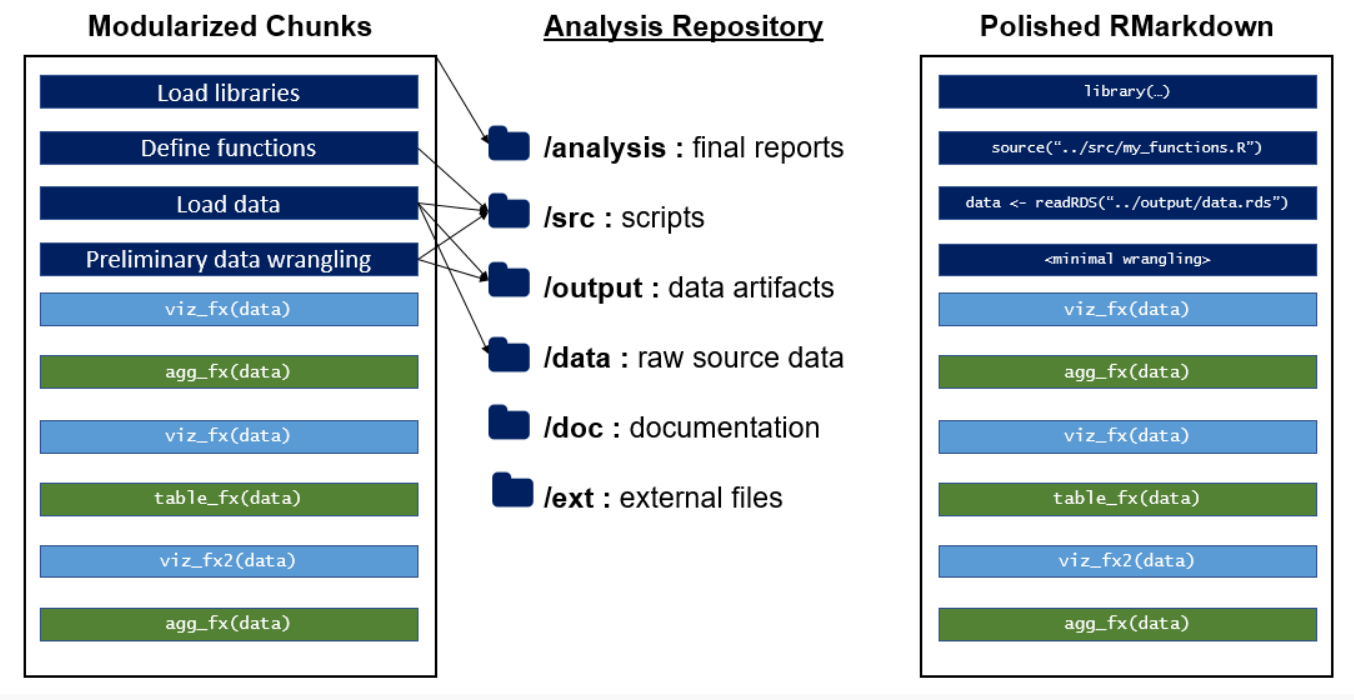
\includegraphics{../external/images/setup_4_markdown_project.PNG}

\url{https://emilyriederer.netlify.com/post/rmarkdown-driven-development/}

\end{frame}

\begin{frame}

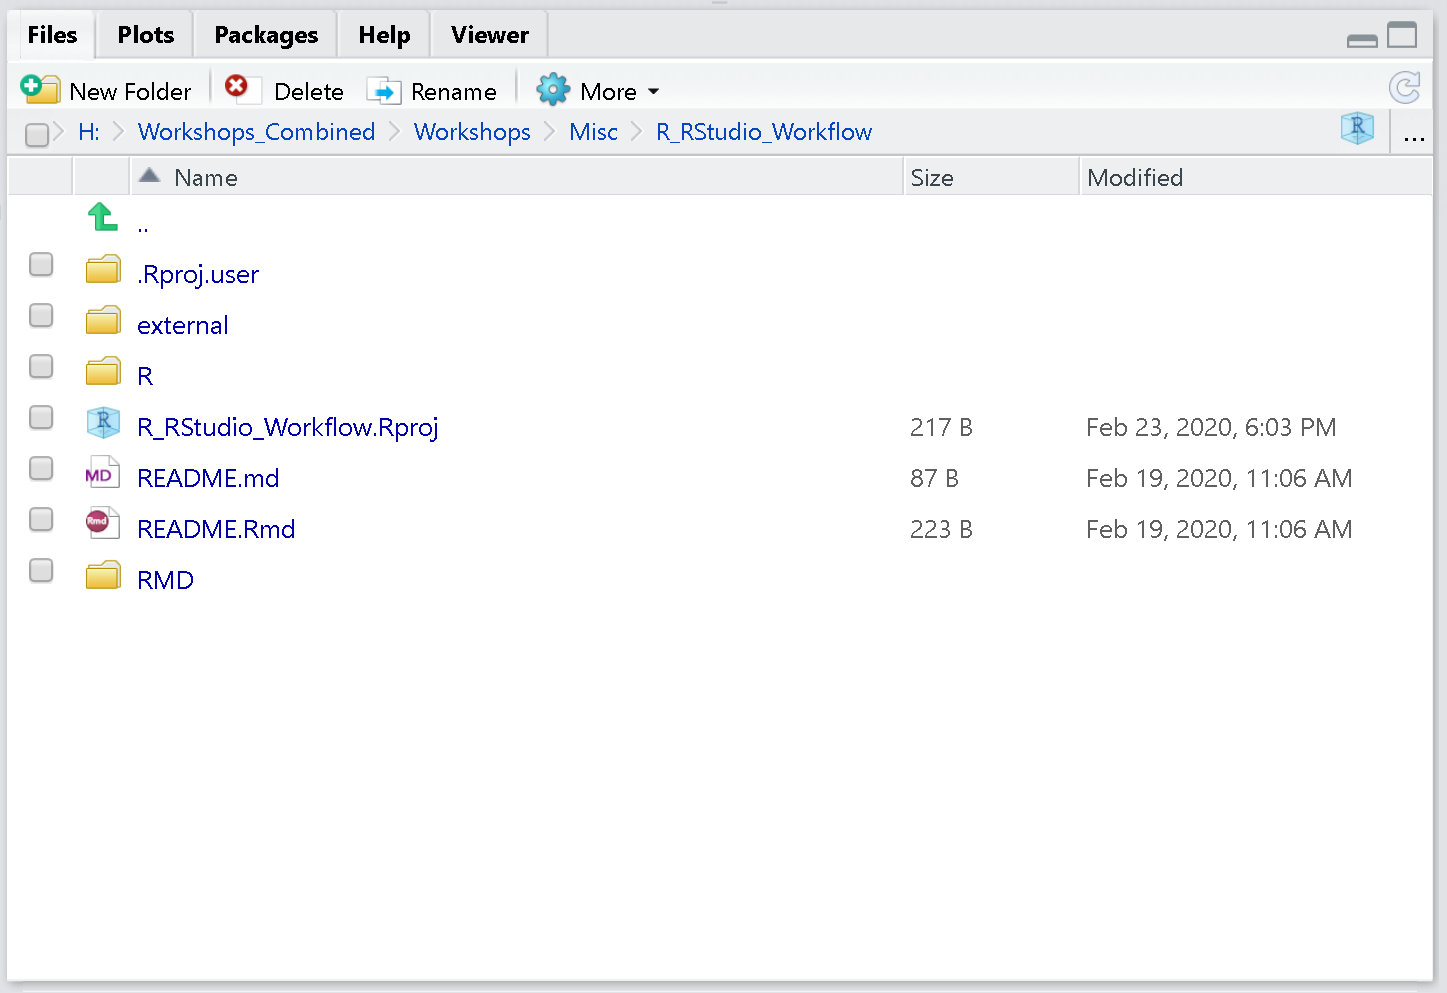
\includegraphics{../external/images/this_project.PNG}

\end{frame}

\begin{frame}{Organize your project folders and markdown}
\protect\hypertarget{organize-your-project-folders-and-markdown}{}

\begin{itemize}[<+->]
\tightlist
\item
  What works for you?
\item
  What works for your organization or team?
\item
  Maximize utility, minimize complexity
\end{itemize}

\end{frame}

\hypertarget{part-1-rstudio-git-r-and-rmarkdown}{%
\section{Part 1: RStudio, Git, R, and
RMarkdown}\label{part-1-rstudio-git-r-and-rmarkdown}}

\hypertarget{rstudio}{%
\subsection{RStudio}\label{rstudio}}

\begin{frame}{RStudio}
\protect\hypertarget{rstudio-1}{}

\begin{itemize}[<+->]
\tightlist
\item
  IDE: Integrated development environment
\item
  RStudio: Does so much

  \begin{itemize}[<+->]
  \tightlist
  \item
    We scratch the surface here
  \end{itemize}
\end{itemize}

\end{frame}

\begin{frame}{RStudio Setup}
\protect\hypertarget{rstudio-setup}{}

\begin{itemize}[<+->]
\tightlist
\item
  Download R and Rstudio

  \begin{itemize}[<+->]
  \tightlist
  \item
    Strongly recommend Microsoft R
    (\url{https://mran.microsoft.com/open})
  \item
    Comes with Intel MKL
  \end{itemize}
\item
  Plain R is fine (\url{https://cran.r-project.org/})

  \begin{itemize}[<+->]
  \tightlist
  \item
    Can relink to faster libraries
  \end{itemize}
\item
  Download RStudio (\url{https://www.rstudio.com/})
\end{itemize}

\end{frame}

\begin{frame}{RStudio Environment}
\protect\hypertarget{rstudio-environment}{}

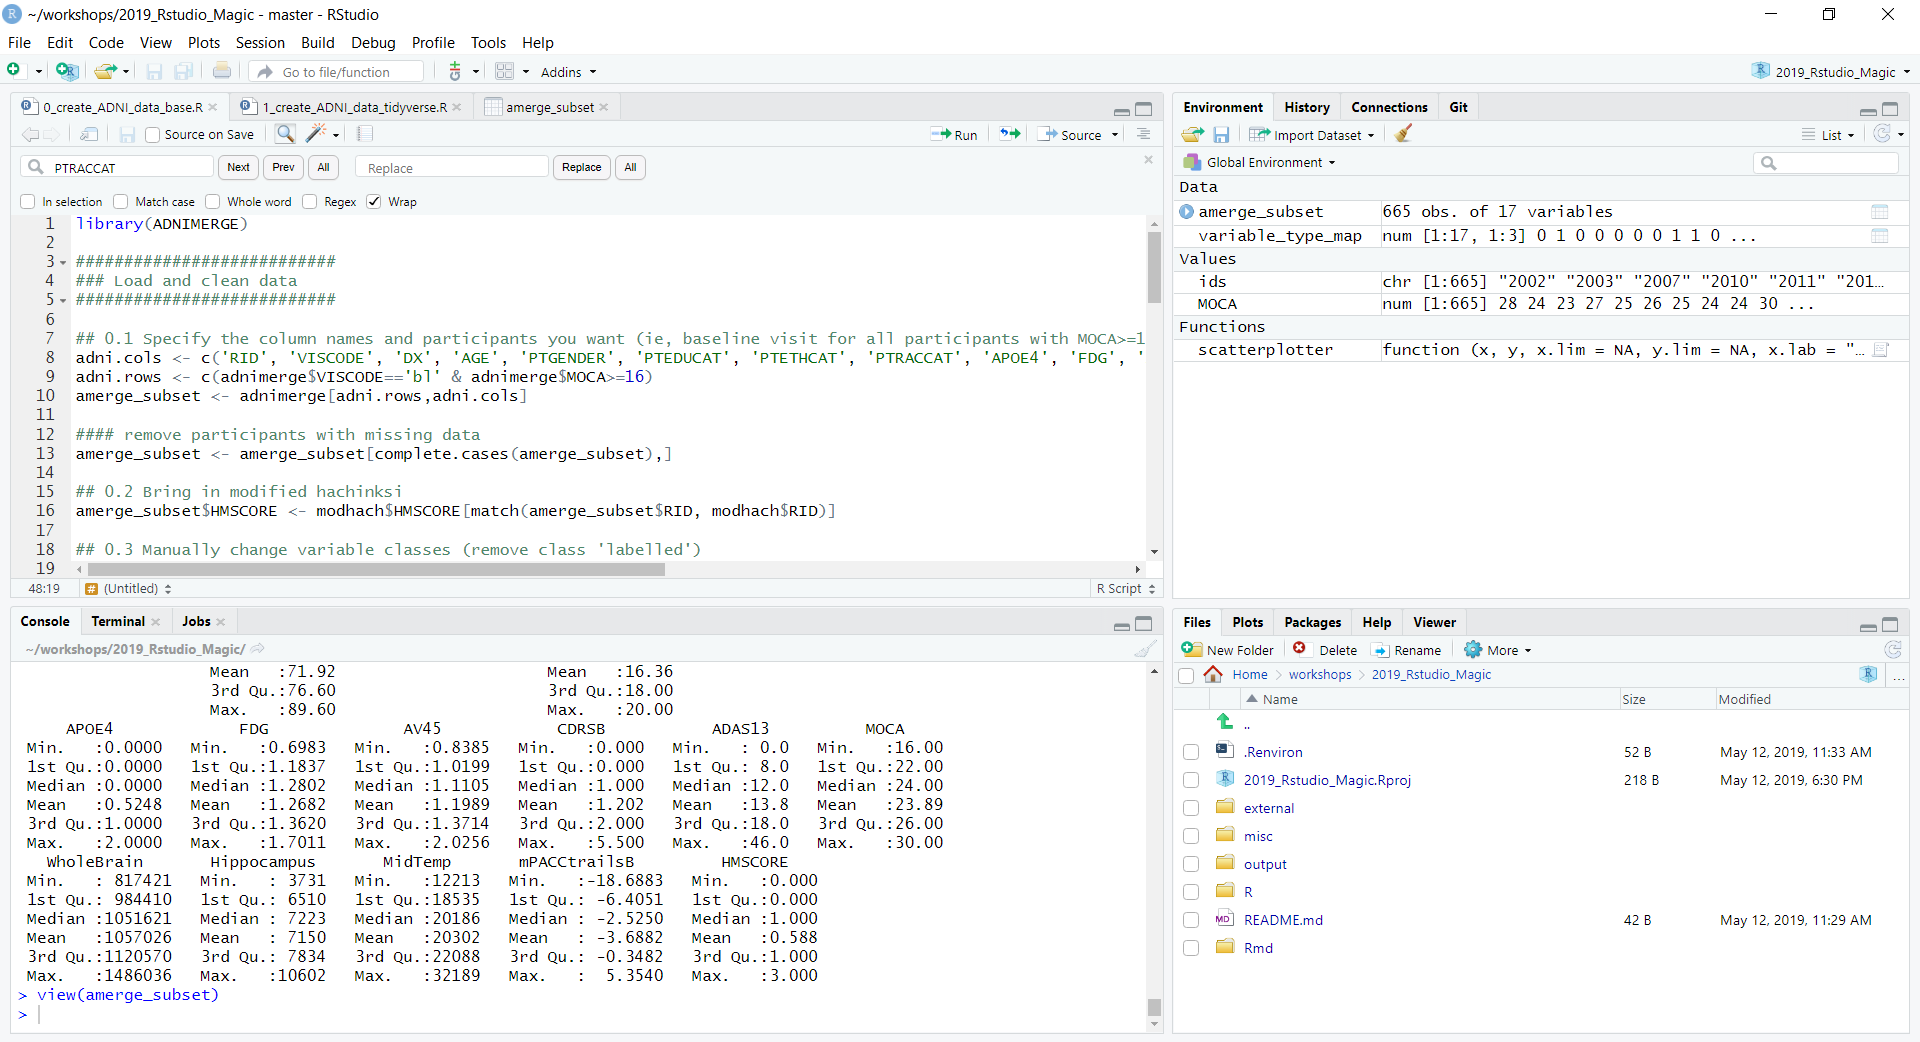
\includegraphics{../external/images/rstudio_terminal_0.PNG}

\end{frame}

\begin{frame}{RStudio Environment}
\protect\hypertarget{rstudio-environment-1}{}

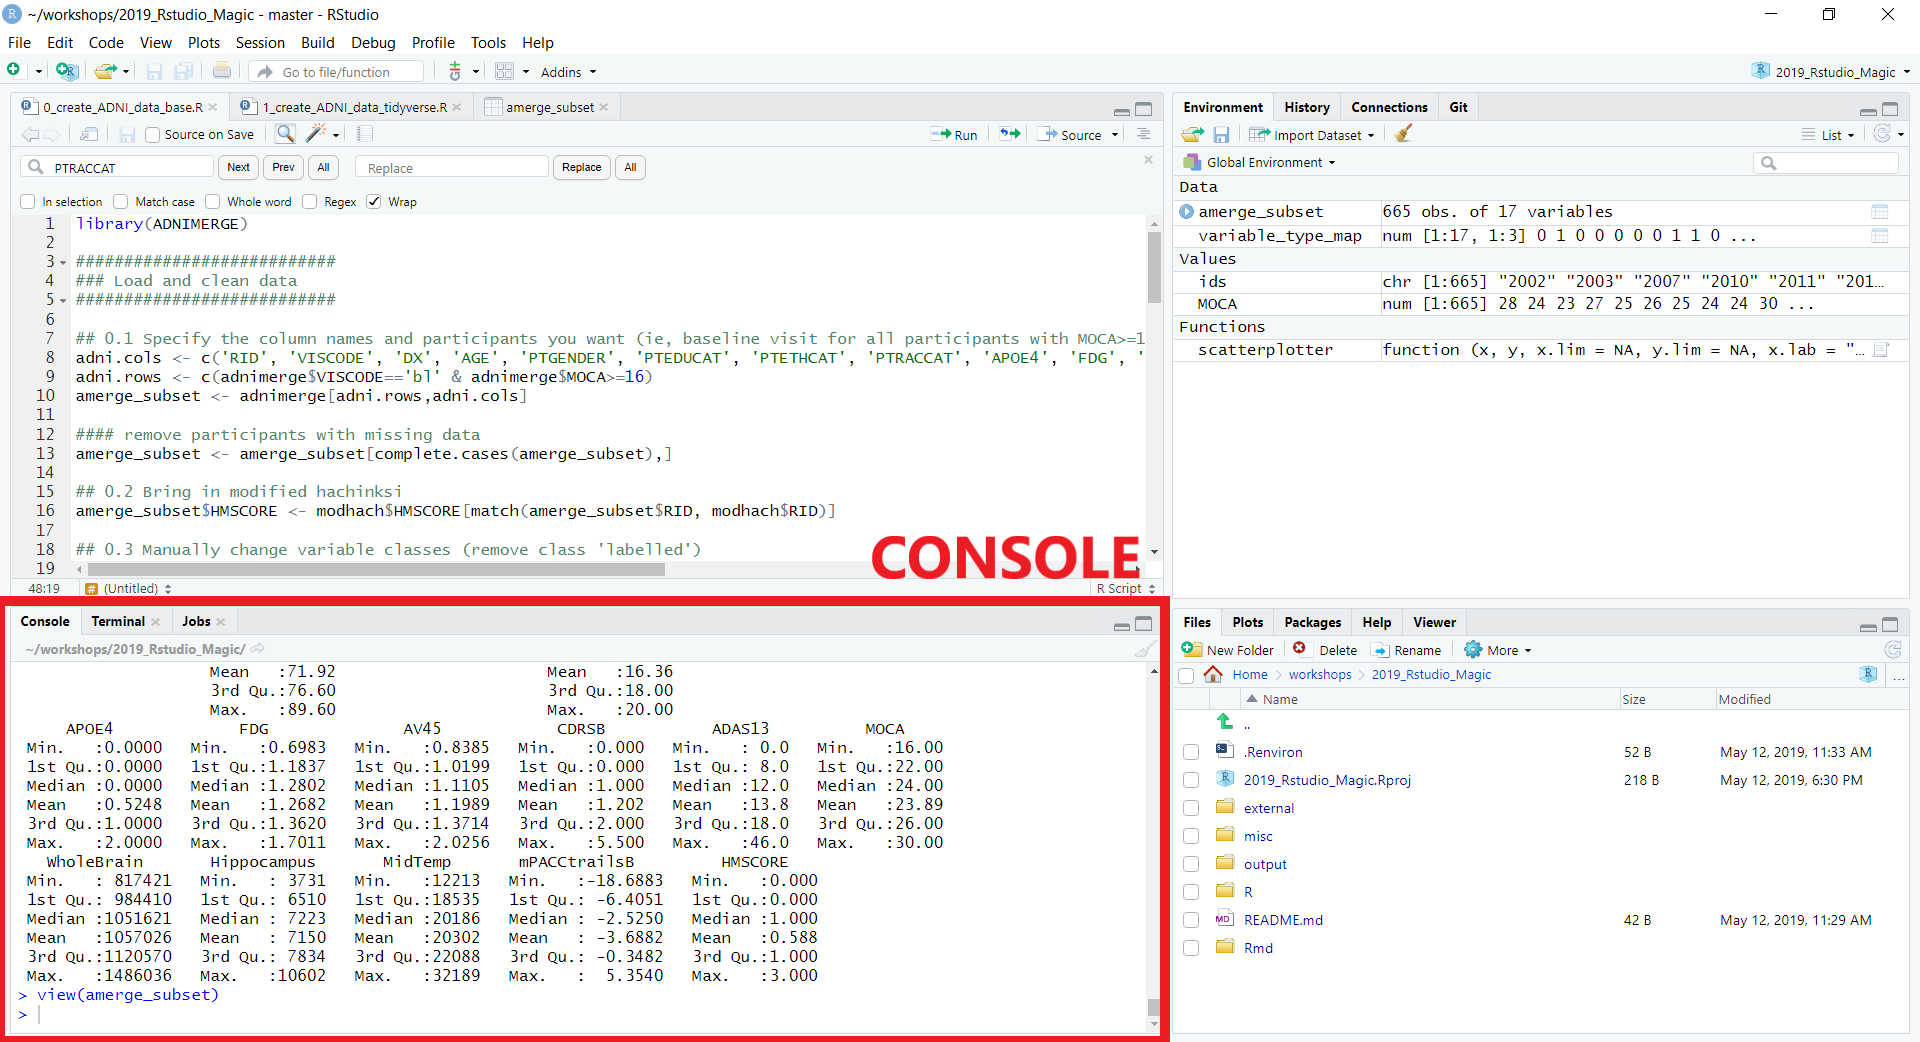
\includegraphics{../external/images/rstudio_terminal_1_CONSOLE.png}

\end{frame}

\begin{frame}{RStudio Environment}
\protect\hypertarget{rstudio-environment-2}{}

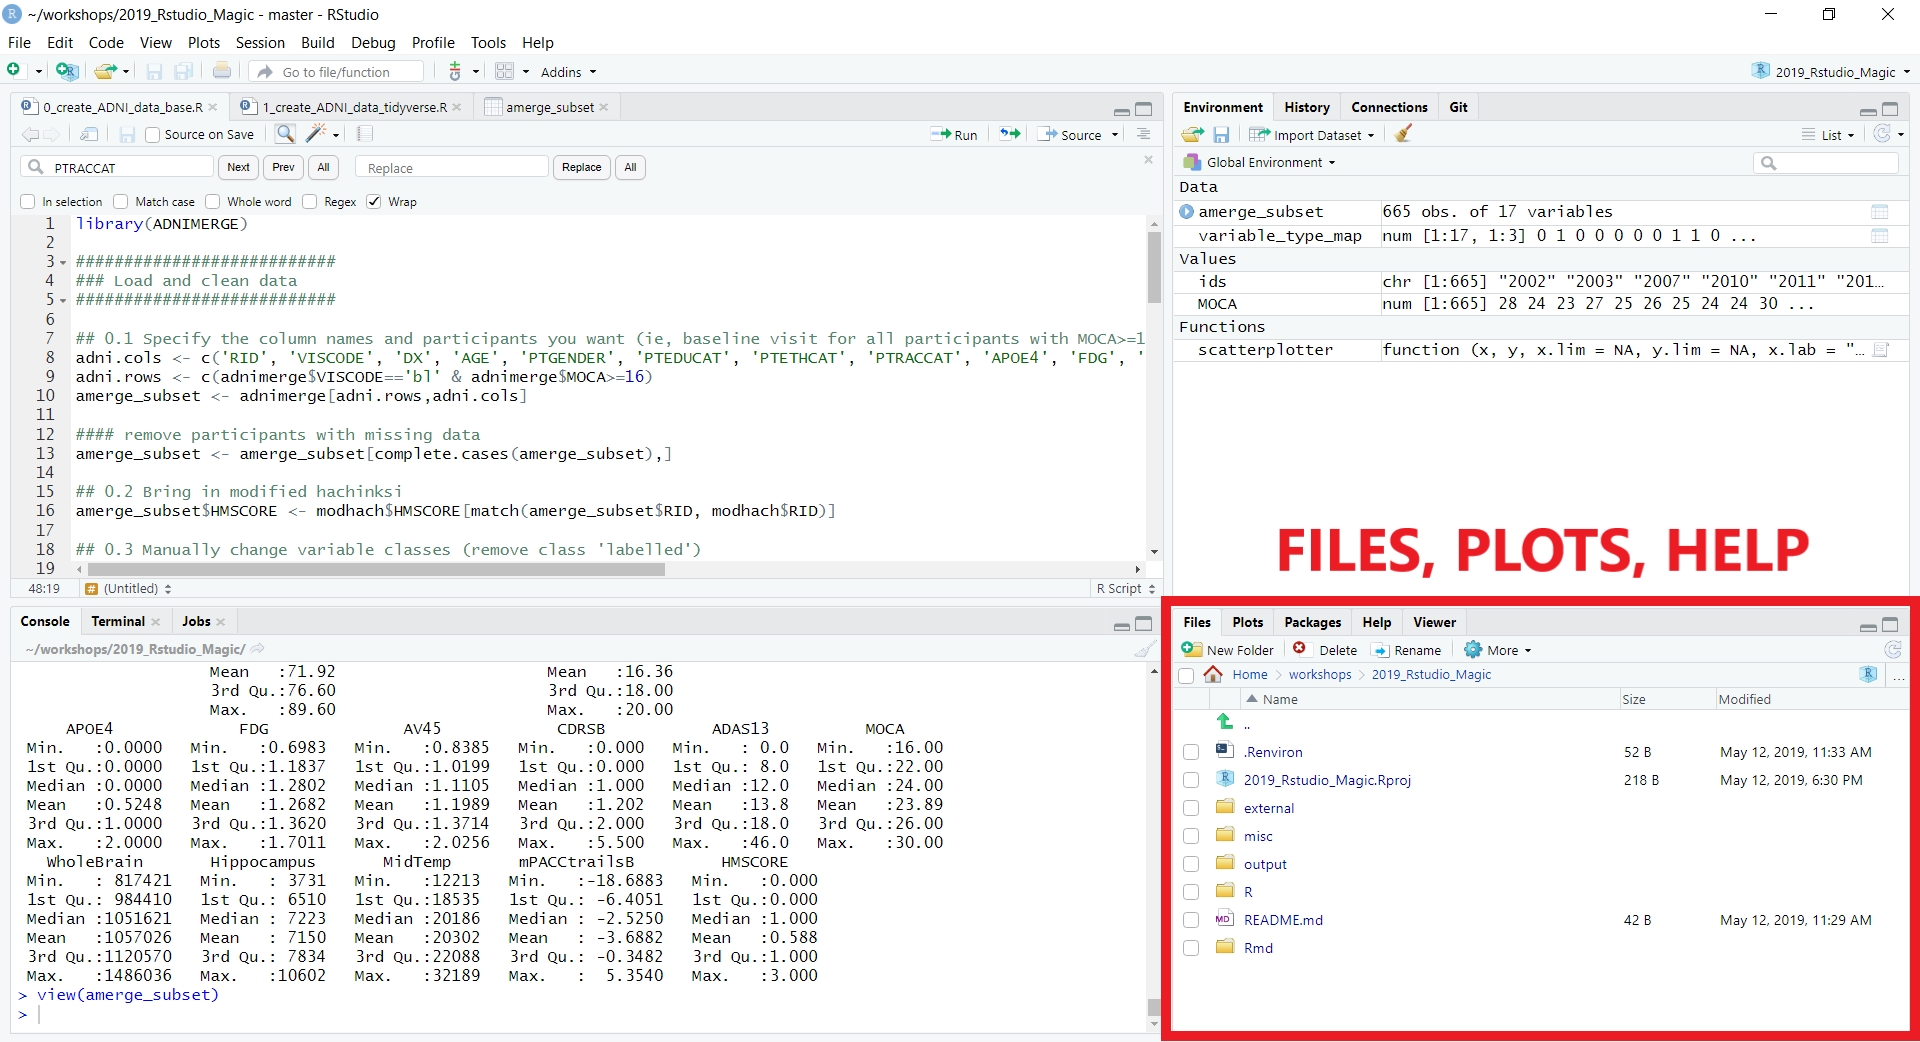
\includegraphics{../external/images/rstudio_terminal_2_FILES.png}

\end{frame}

\begin{frame}{RStudio Environment}
\protect\hypertarget{rstudio-environment-3}{}

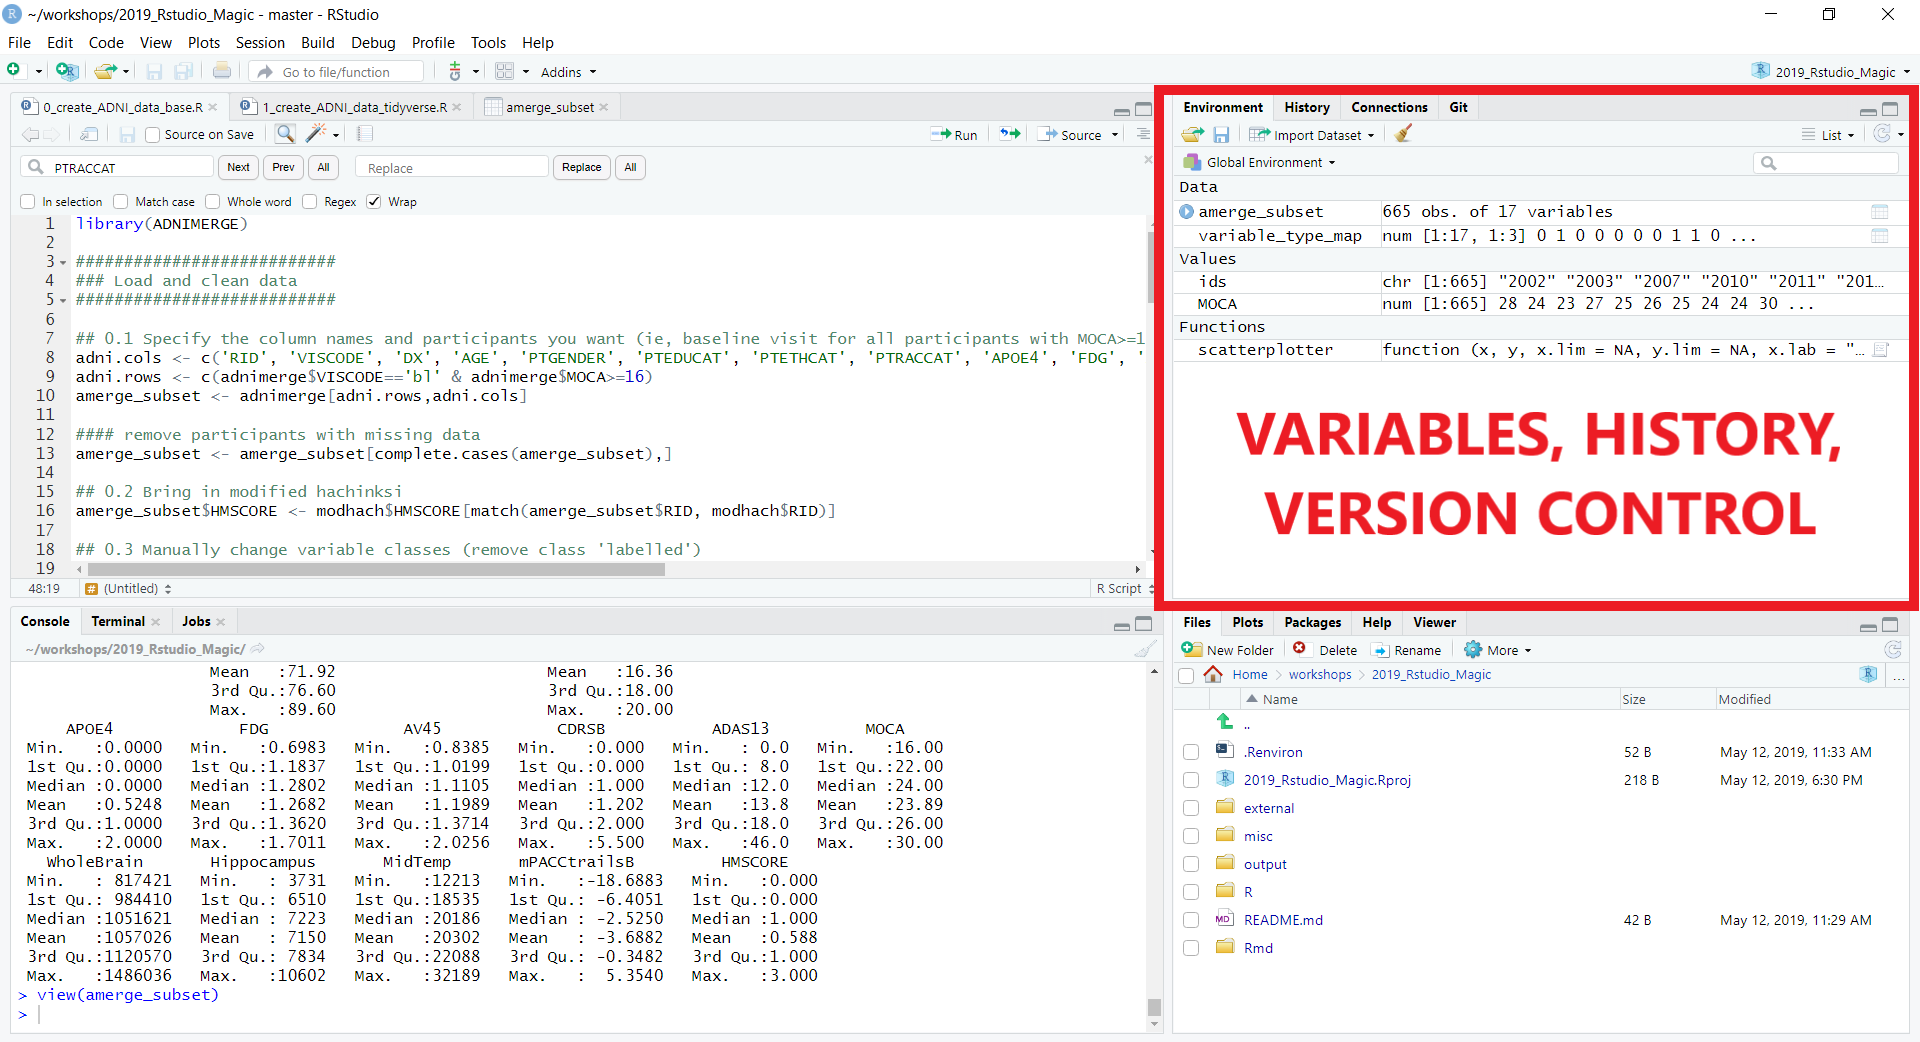
\includegraphics{../external/images/rstudio_terminal_3_ENV.png}

\end{frame}

\begin{frame}{RStudio Environment}
\protect\hypertarget{rstudio-environment-4}{}

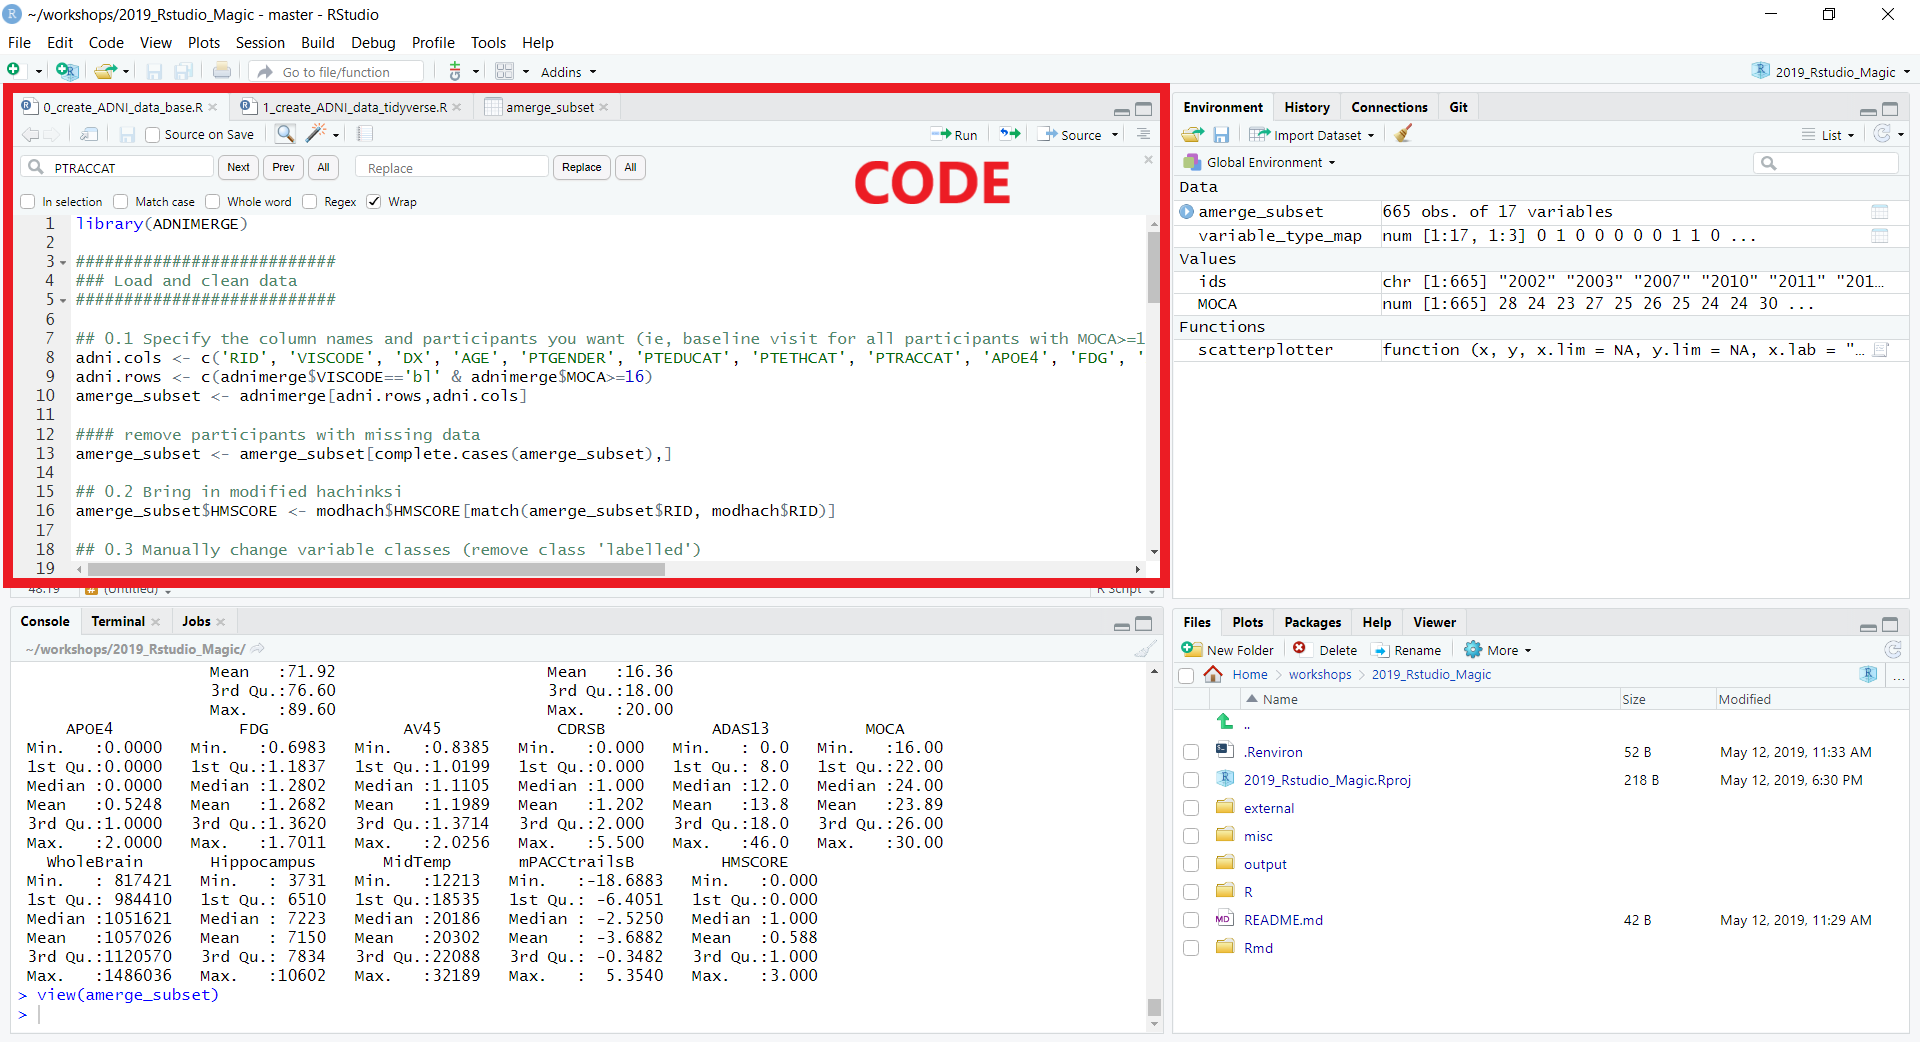
\includegraphics{../external/images/rstudio_terminal_4_CODE.png}

\end{frame}

\begin{frame}{RStudio Environment}
\protect\hypertarget{rstudio-environment-5}{}

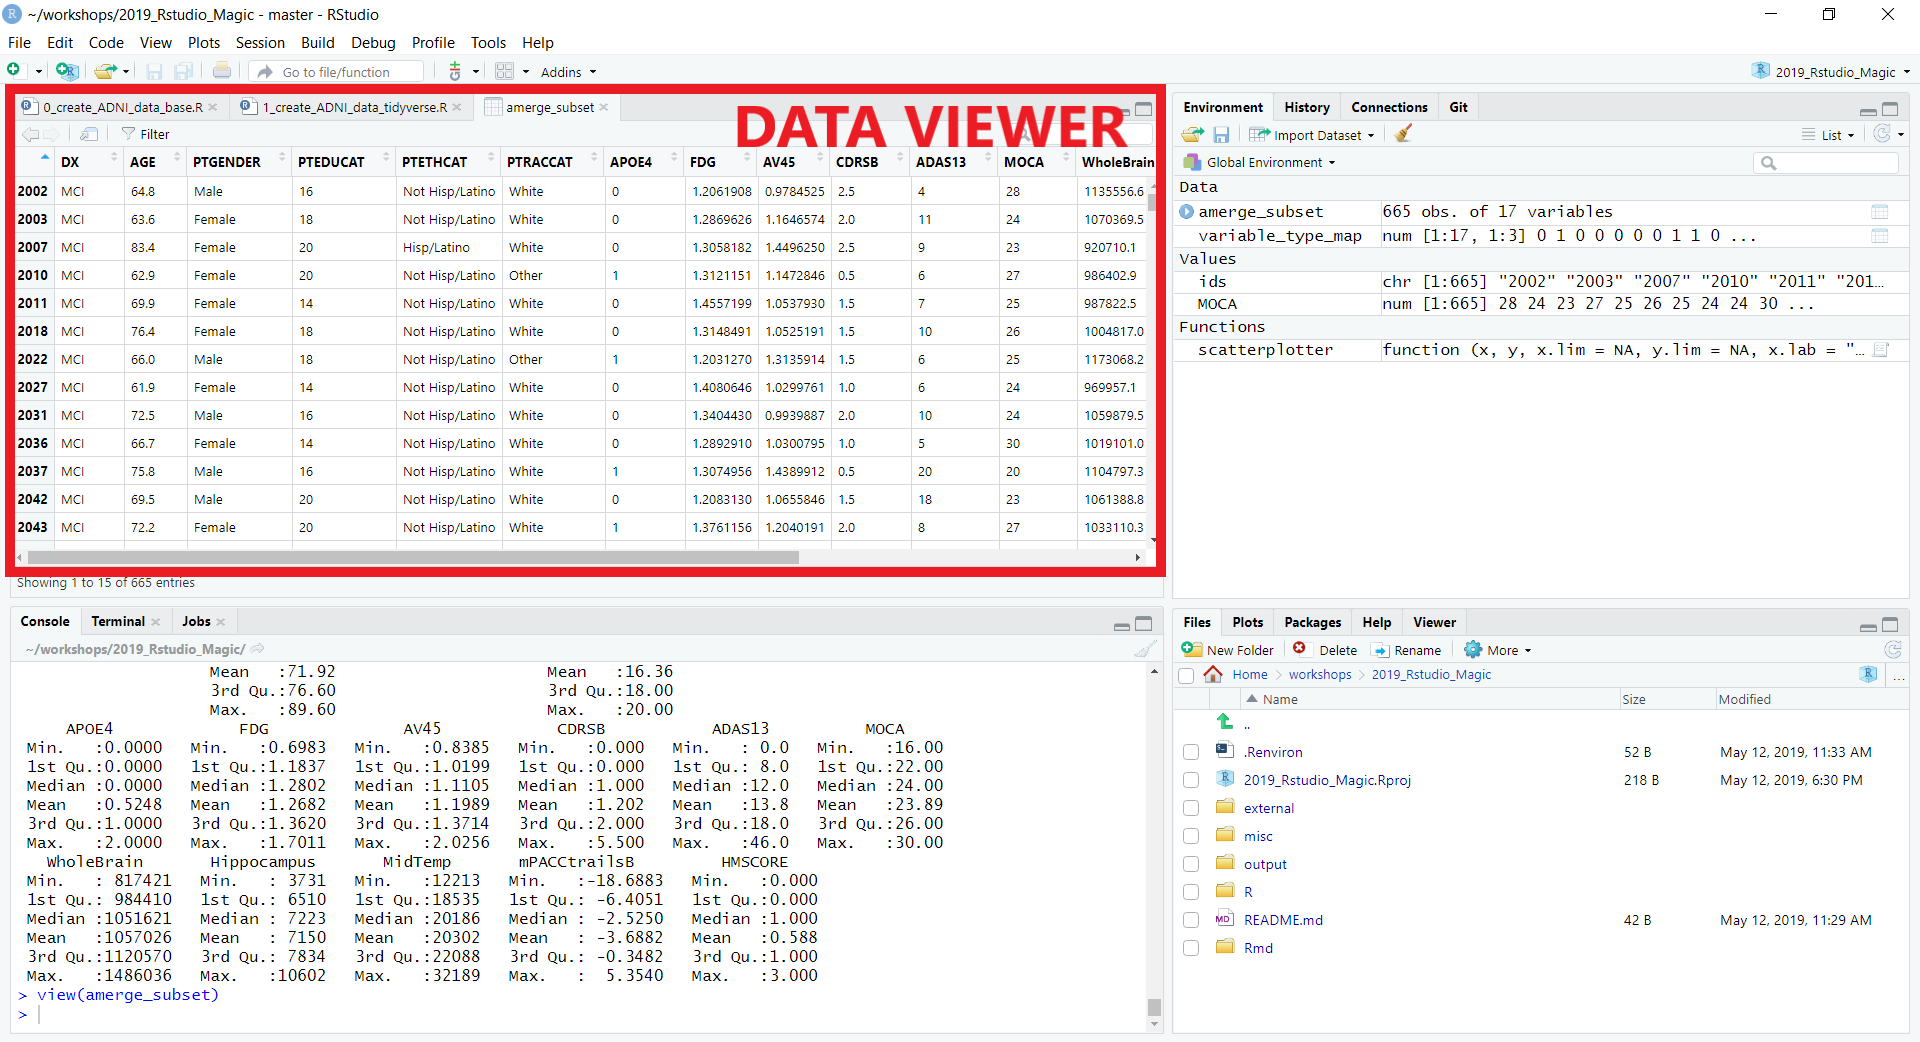
\includegraphics{../external/images/rstudio_terminal_5_DATA.png}

\end{frame}

\begin{frame}{RStudio is more}
\protect\hypertarget{rstudio-is-more}{}

\begin{itemize}[<+->]
\tightlist
\item
  Not just an IDE (integrated development environment)
\item
  A company
\item
  A community
\item
  A conference
\item
  A centralized resource
\end{itemize}

\end{frame}

\begin{frame}{RStudio Resources}
\protect\hypertarget{rstudio-resources}{}

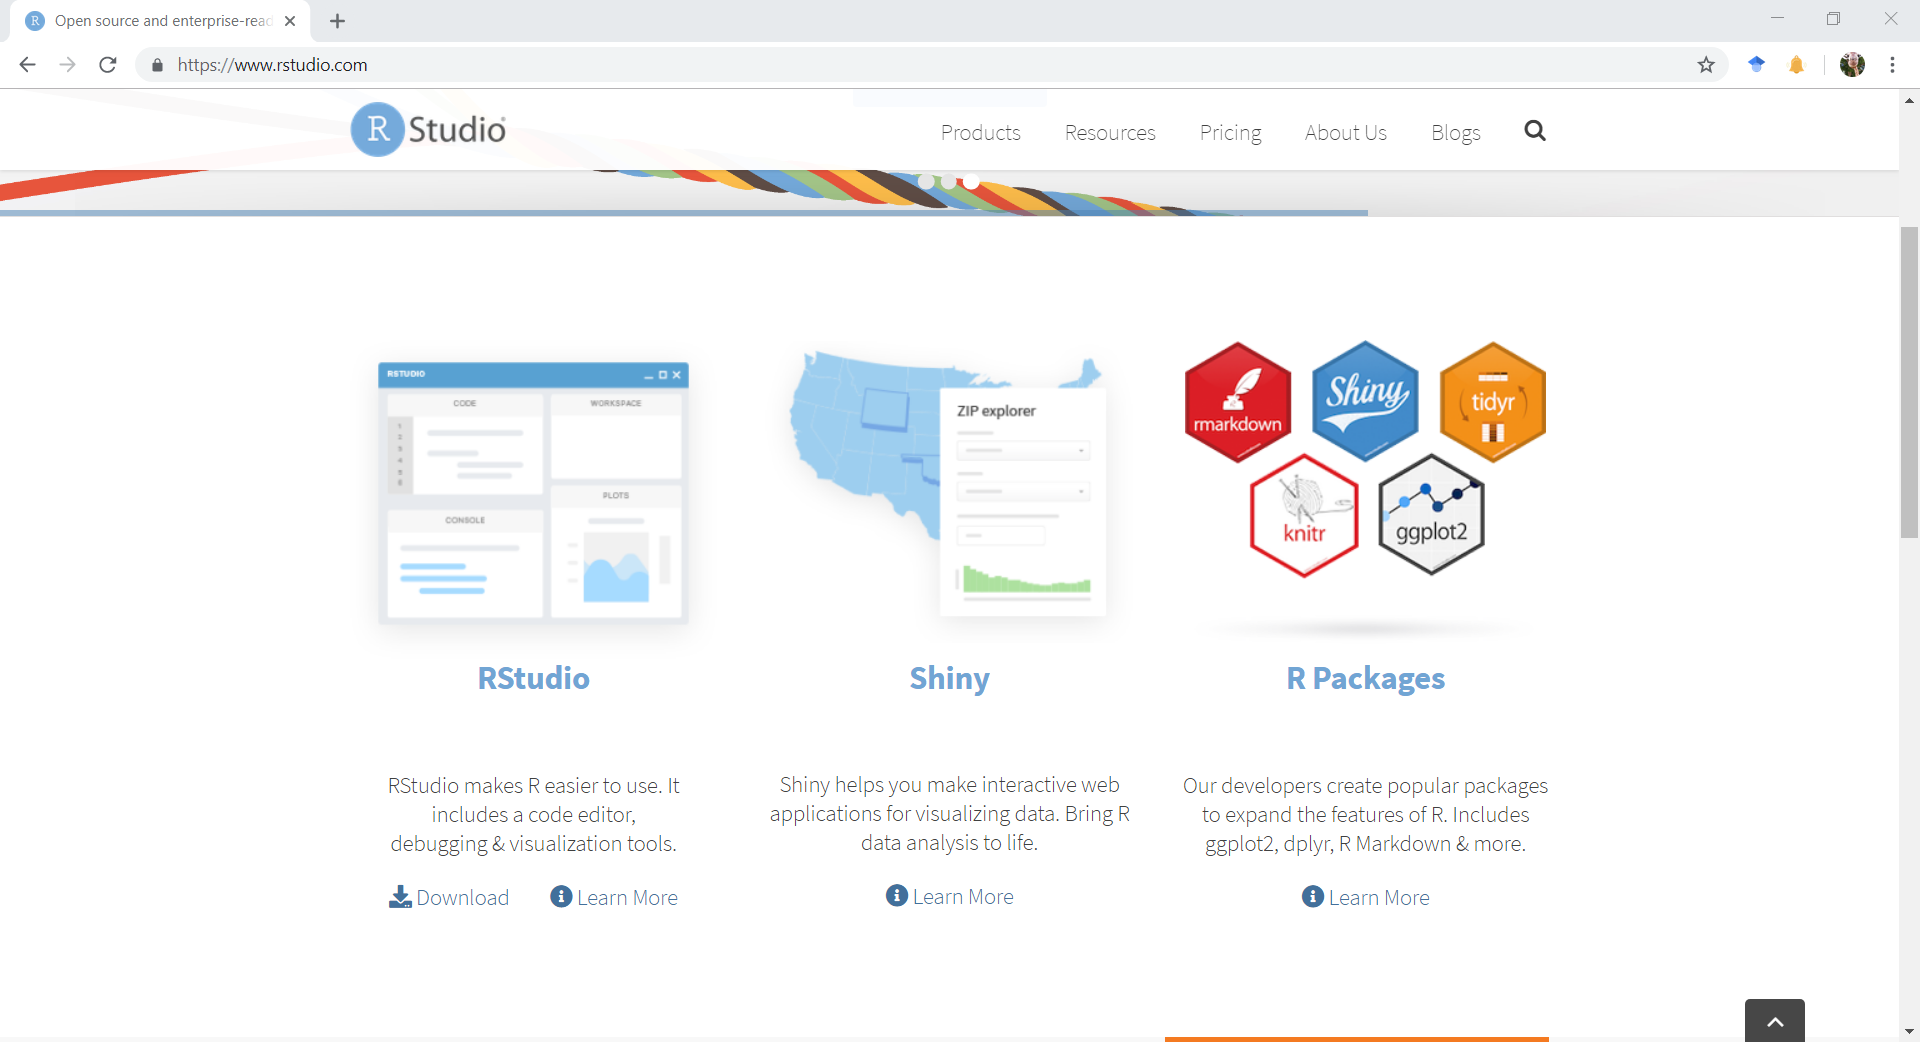
\includegraphics{../external/images/rstudio_dot_com_1_main.PNG}

\end{frame}

\begin{frame}{RStudio Resources}
\protect\hypertarget{rstudio-resources-1}{}

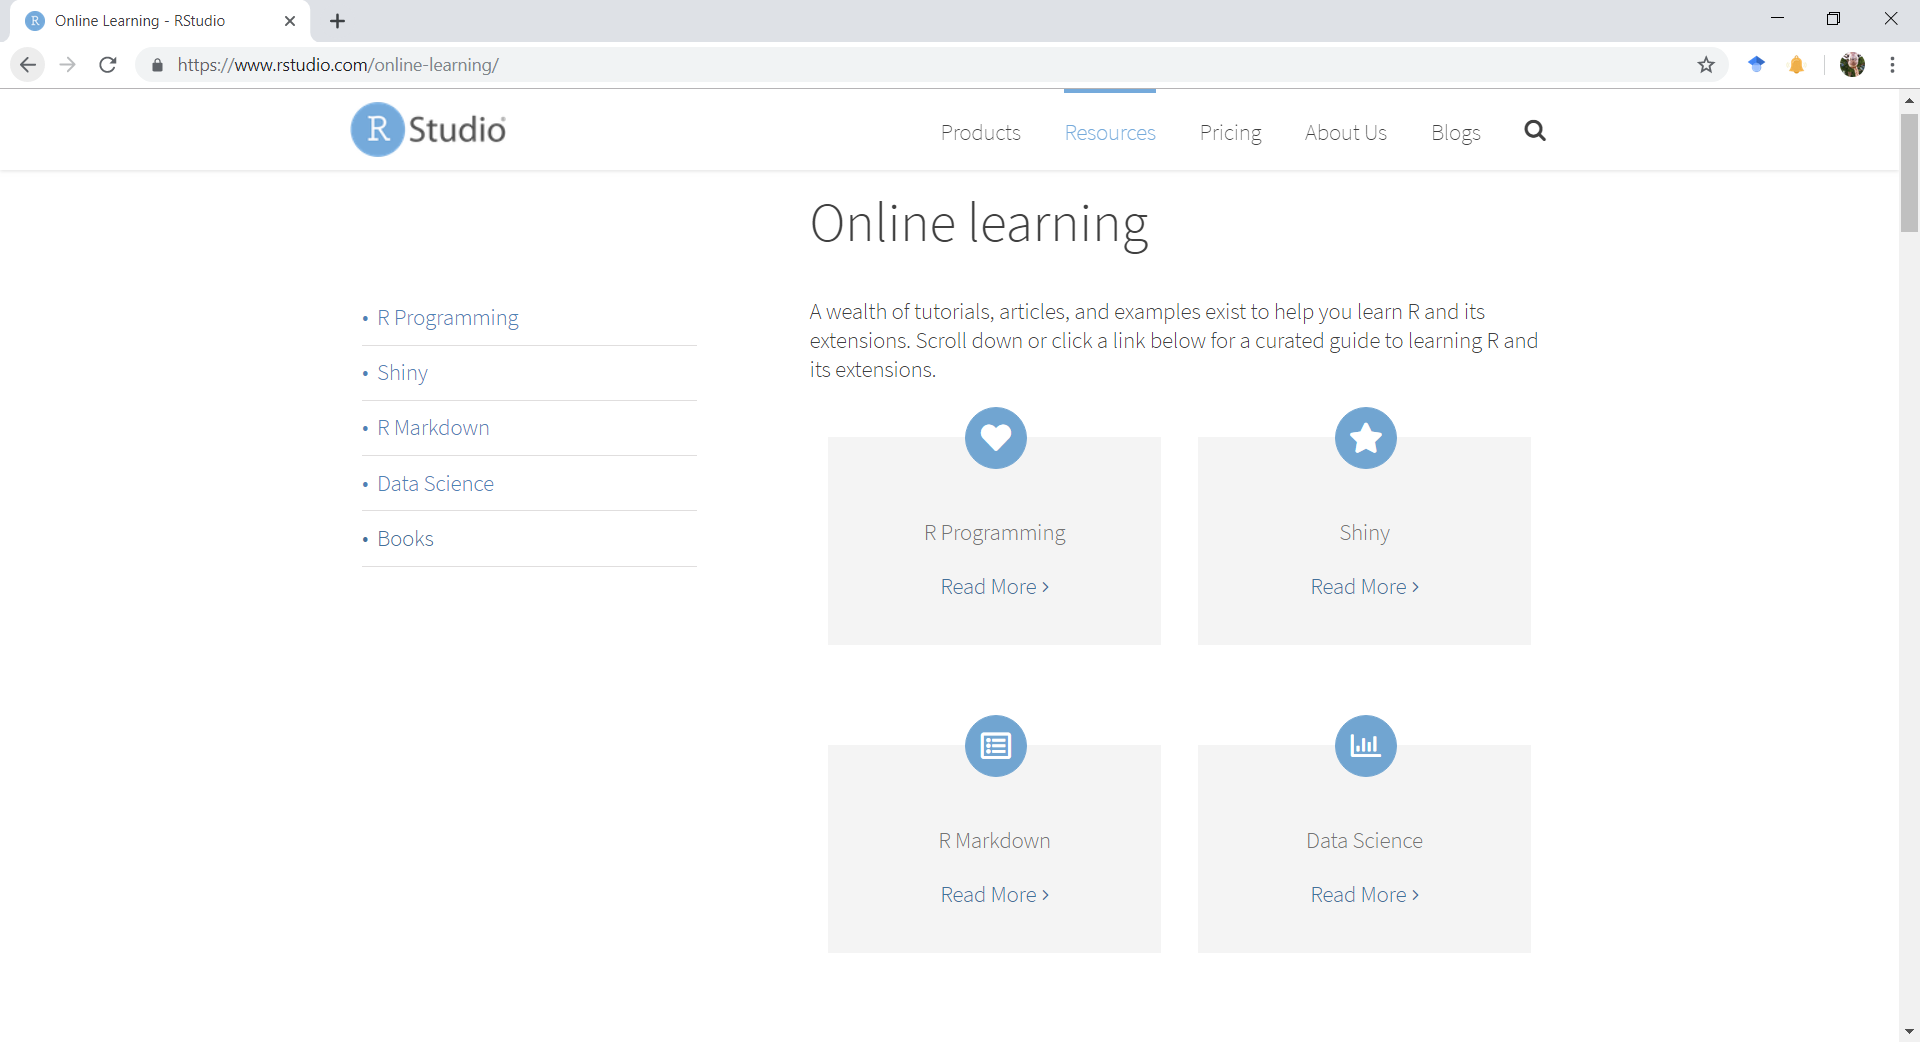
\includegraphics{../external/images/rstudio_dot_com_2_learning.PNG}

\end{frame}

\begin{frame}{RStudio Resources}
\protect\hypertarget{rstudio-resources-2}{}

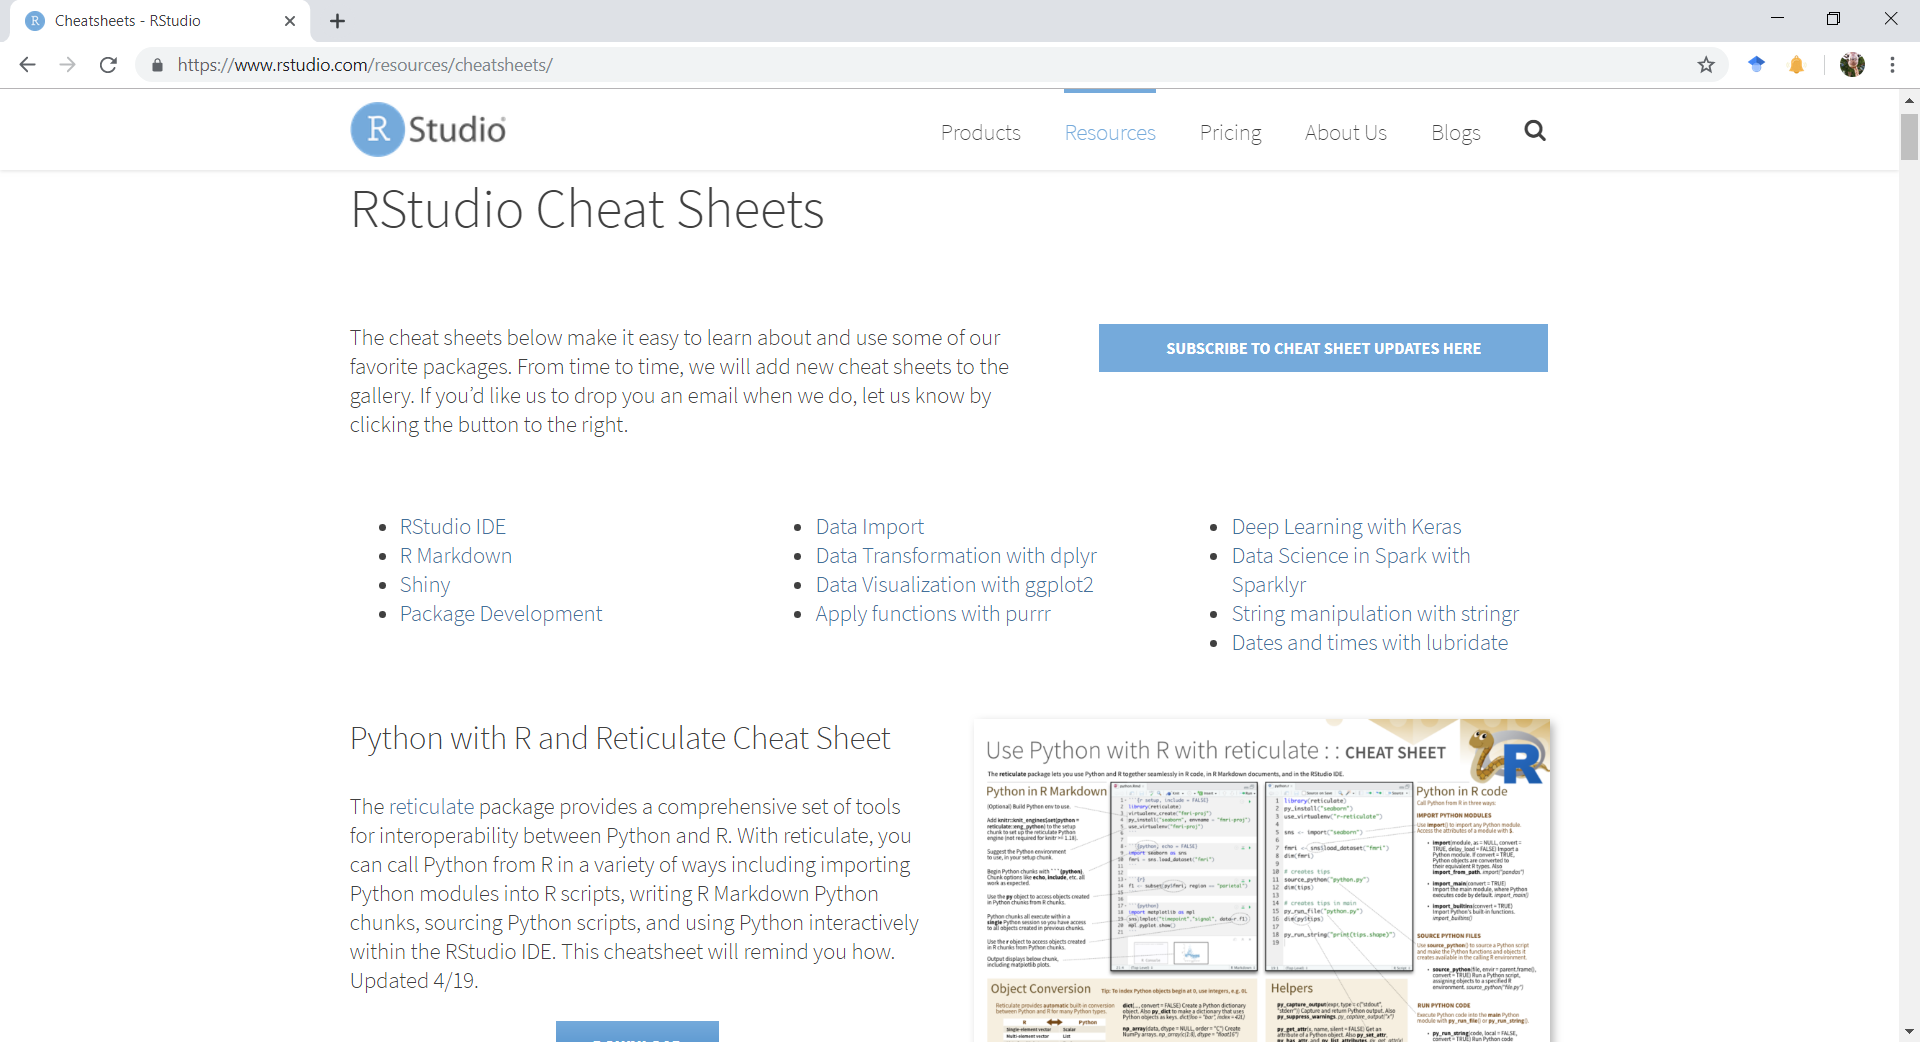
\includegraphics{../external/images/rstudio_dot_com_3_cheats.PNG}

\end{frame}

\begin{frame}{RStudio Setup}
\protect\hypertarget{rstudio-setup-1}{}

\begin{itemize}[<+->]
\tightlist
\item
  For set up:
  \url{https://jennybc.github.io/2014-05-12-ubc/r-setup.html}
\item
  For R projects, see

  \begin{itemize}[<+->]
  \tightlist
  \item
    \url{https://support.rstudio.com/hc/en-us/articles/200526207-Using-Projects}
  \item
    \url{https://r4ds.had.co.nz/workflow-projects.html}
  \end{itemize}
\end{itemize}

\end{frame}

\begin{frame}{R Projects}
\protect\hypertarget{r-projects}{}

Compartmentalize \& collaborate:

\begin{itemize}[<+->]
\tightlist
\item
  RStudio projects

  \begin{itemize}[<+->]
  \tightlist
  \item
    ``RStudio projects make it straightforward to divide your work into
    multiple contexts, each with their own working directory, workspace,
    history, and source documents.''
  \item
    specific projects
  \item
    R package development
  \item
    cloning from (e.g., Git) repos
  \end{itemize}
\end{itemize}

\end{frame}

\begin{frame}

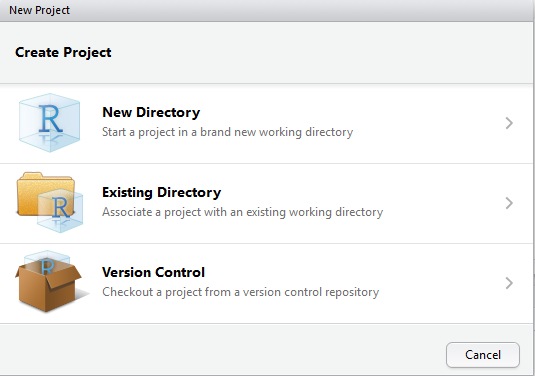
\includegraphics[width=0.75\textwidth,height=\textheight]{../external/images/setup_2_rstudio_project.PNG}

\end{frame}

\begin{frame}

.Rproj files: just a text file with some parameters for start up
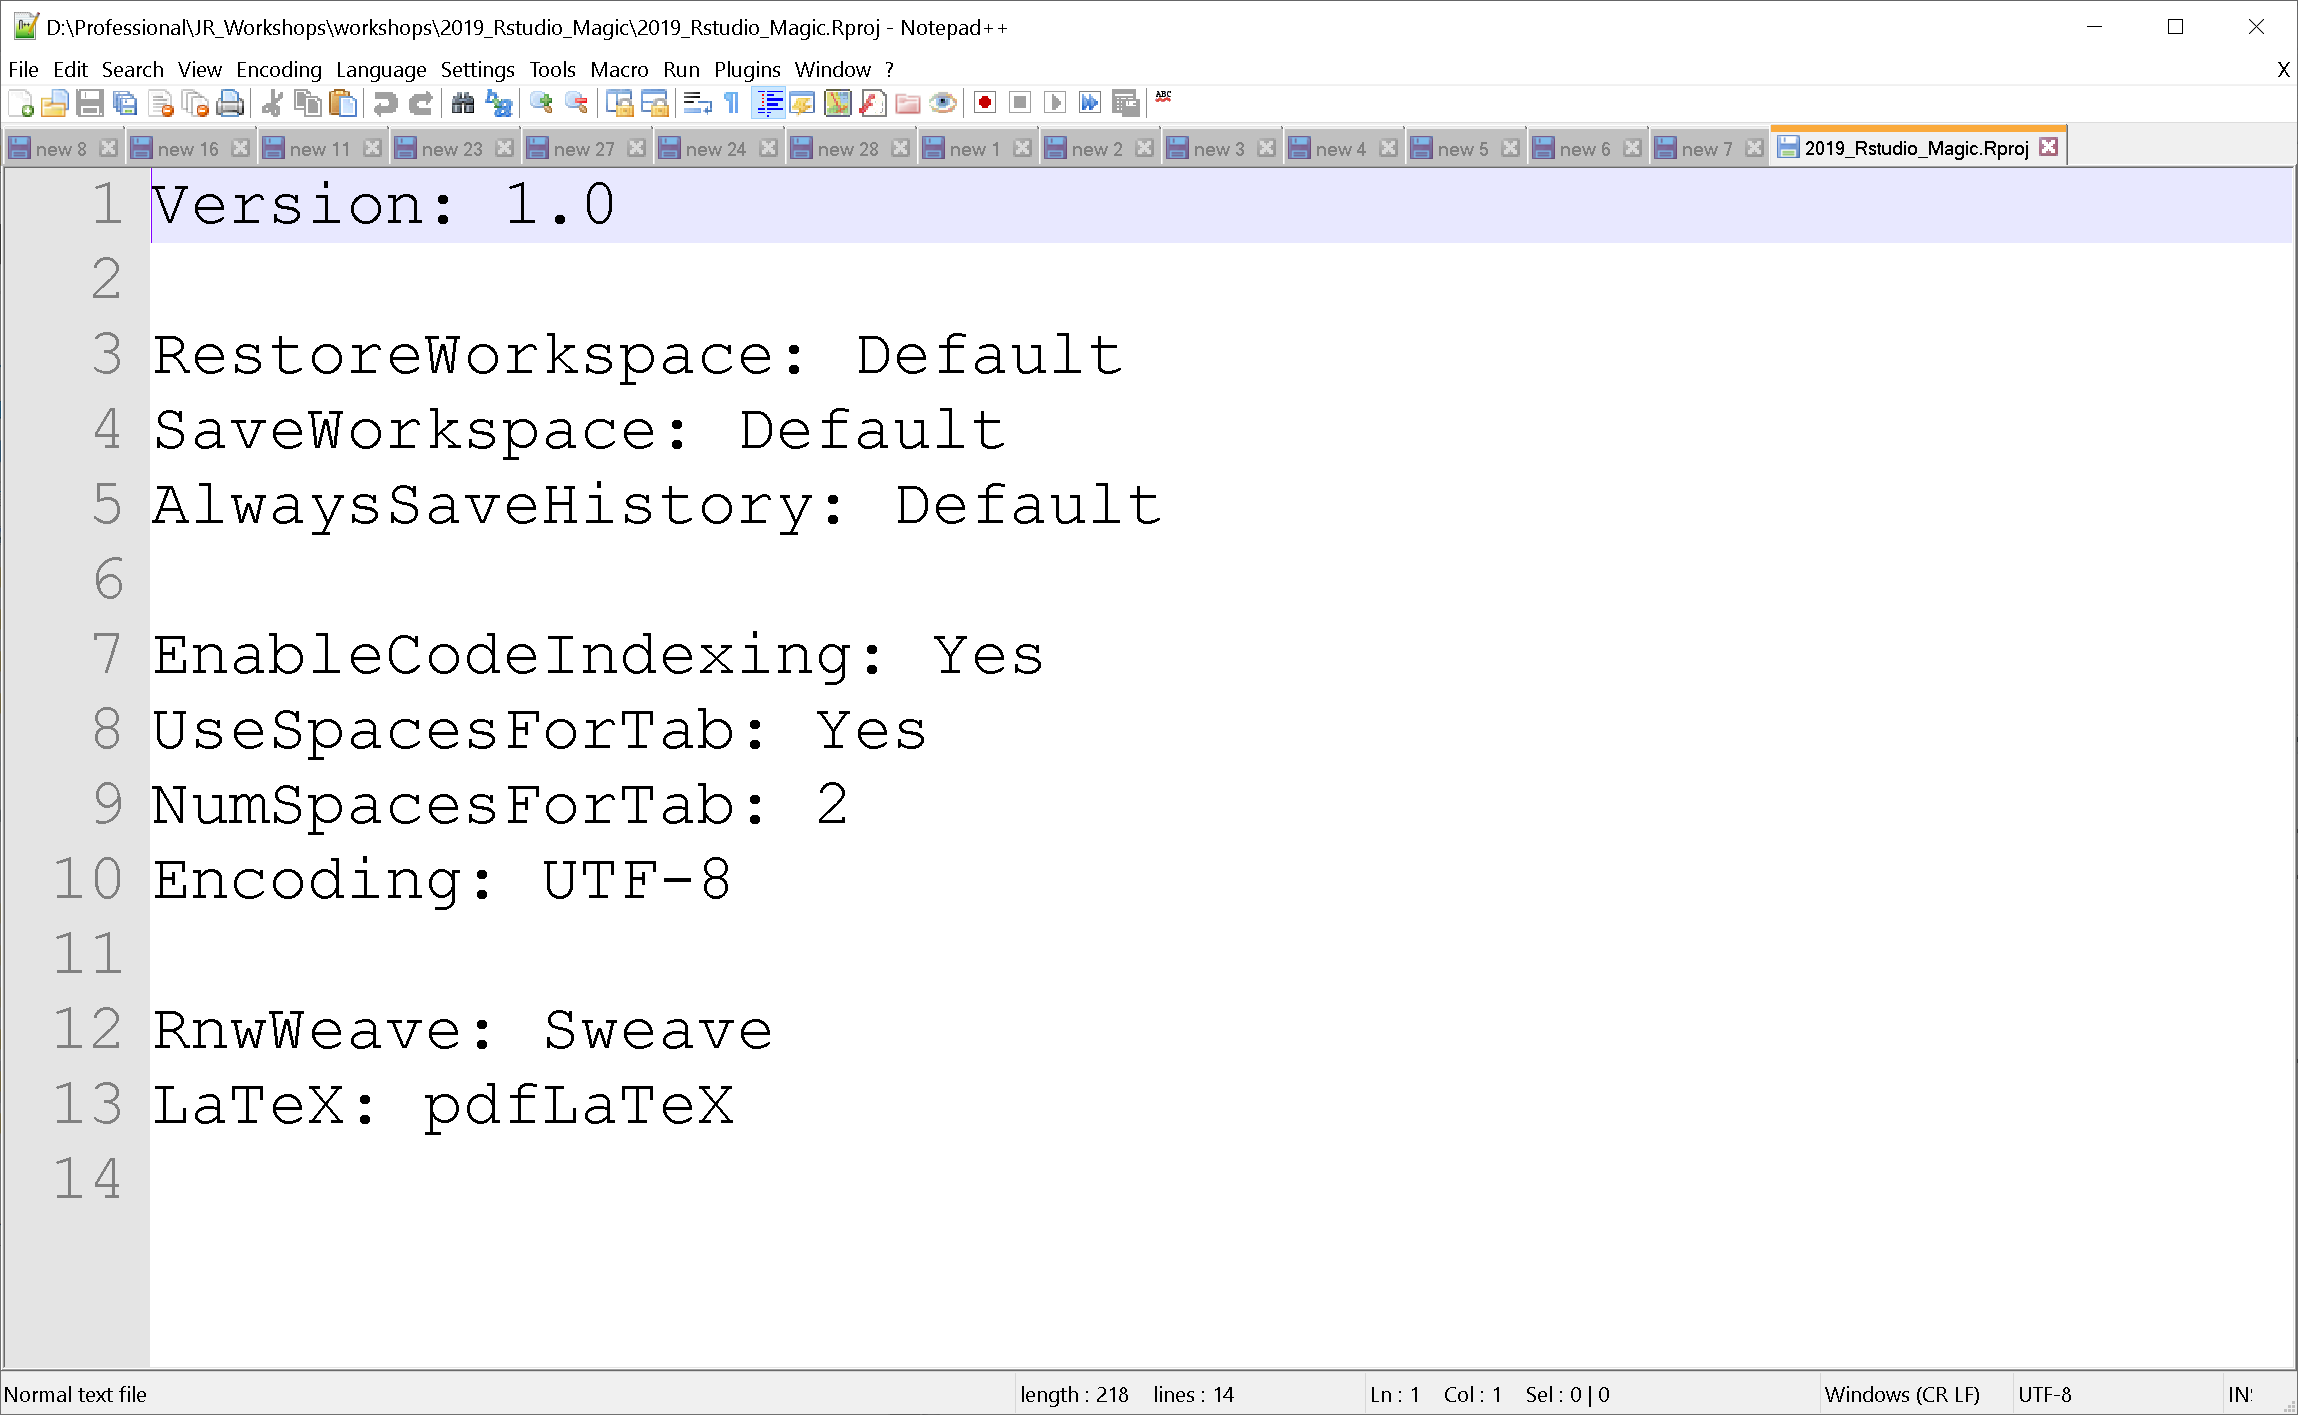
\includegraphics[width=0.5\textwidth,height=\textheight]{../external/images/Rproj_inside.PNG}

\end{frame}

\begin{frame}

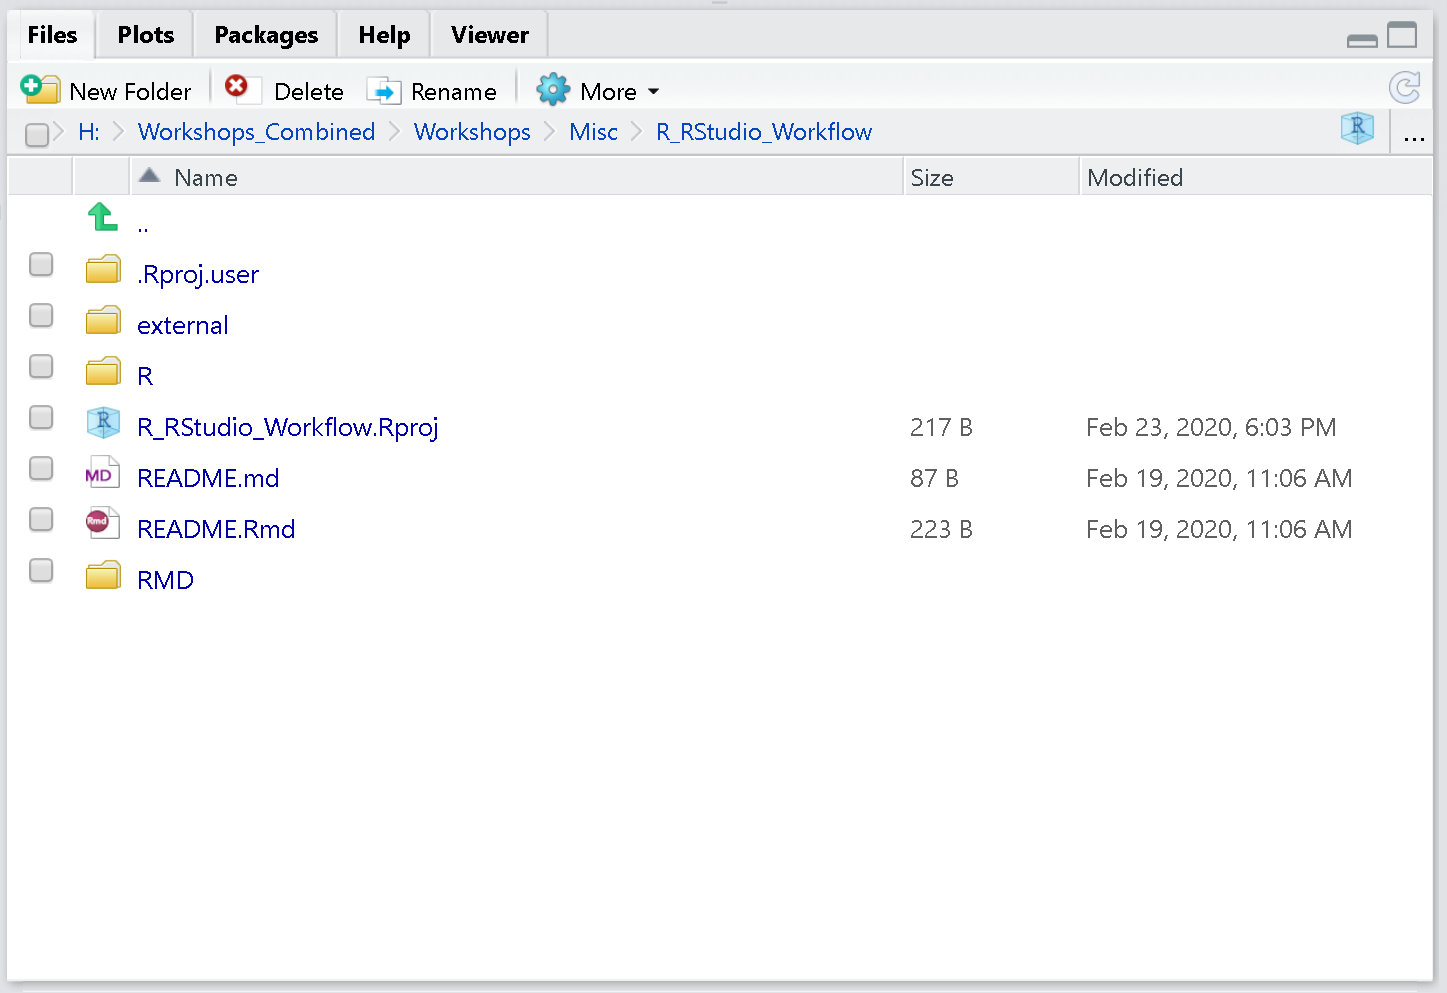
\includegraphics{../external/images/this_project.PNG}

\end{frame}

\hypertarget{git}{%
\subsection{Git}\label{git}}

\begin{frame}{What is Git?}
\protect\hypertarget{what-is-git}{}

\begin{itemize}[<+->]
\tightlist
\item
  Version control (like SVN, a.k.a. subversion)
\item
  Traditionally for developers/software
\item
  Now more common to ``track changes''
\end{itemize}

\end{frame}

\begin{frame}

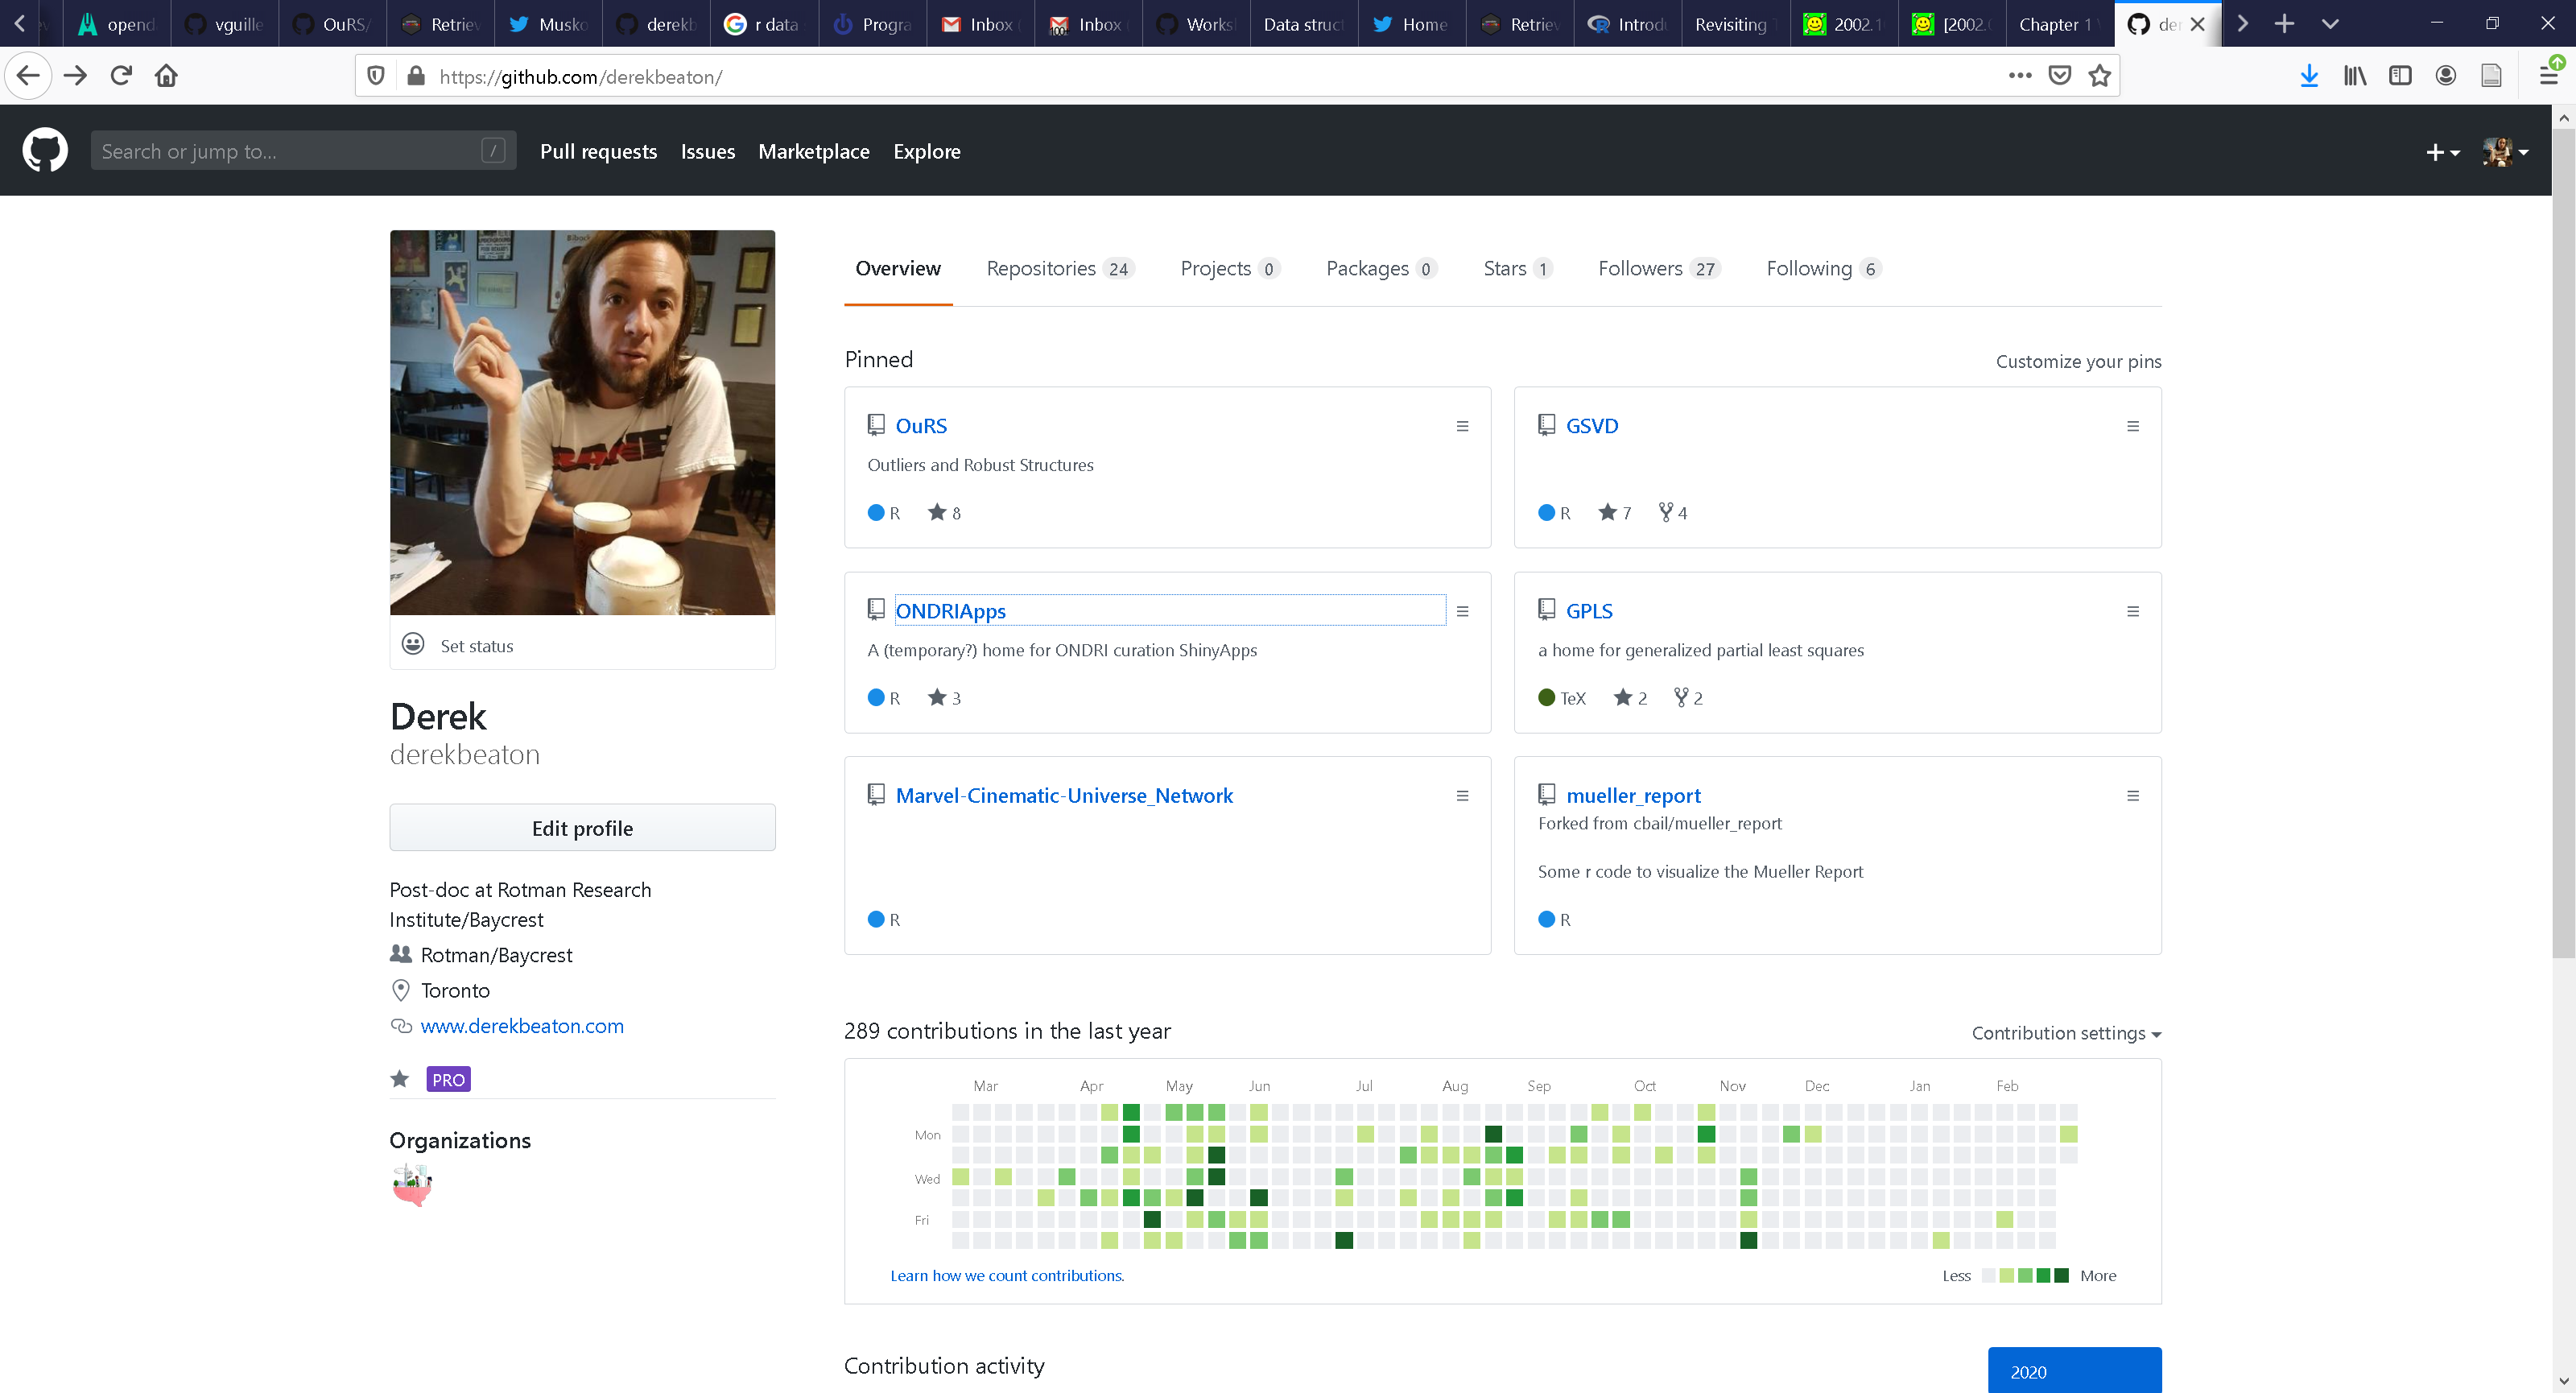
\includegraphics[width=0.9\textwidth,height=\textheight]{../external/images/DB_GIT.PNG}

\end{frame}

\begin{frame}

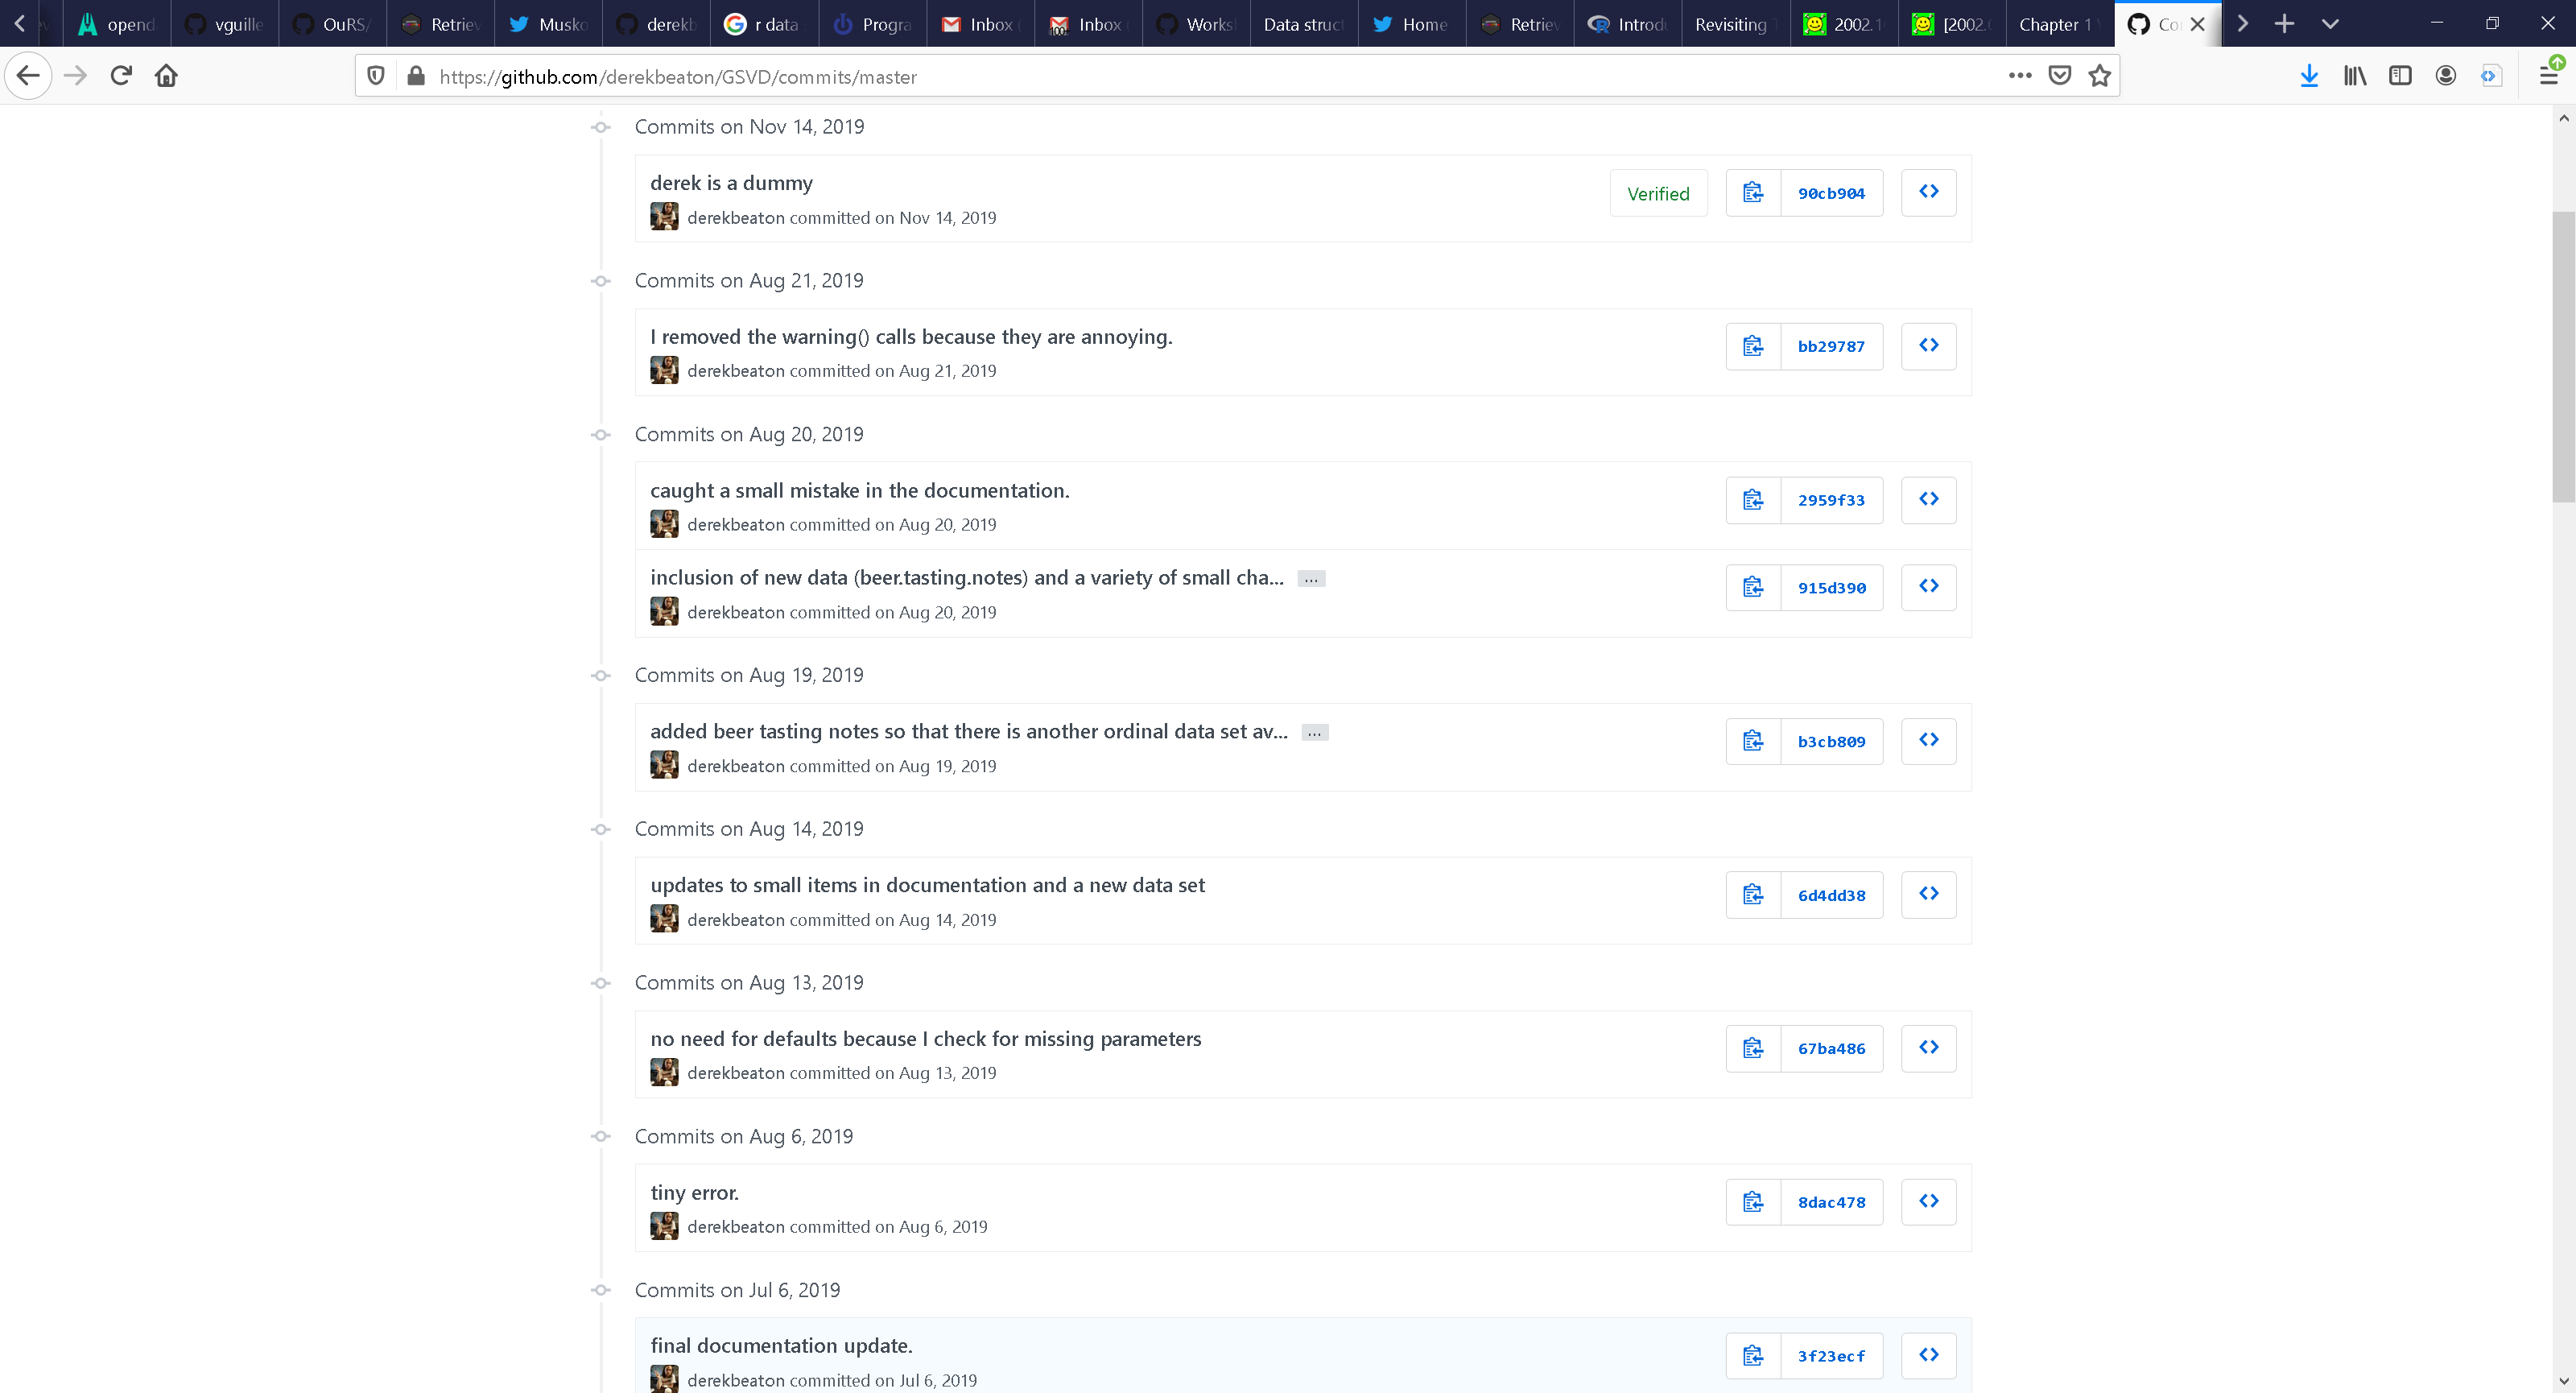
\includegraphics[width=0.9\textwidth,height=\textheight]{../external/images/DB_GSVD_History.PNG}

\end{frame}

\begin{frame}{Github}
\protect\hypertarget{github}{}

\begin{itemize}[<+->]
\tightlist
\item
  As students: You can get free pro accounts
\item
  And you really really should
\item
  \url{https://education.github.com/pack}
\end{itemize}

\end{frame}

\begin{frame}{Git \& R Projects}
\protect\hypertarget{git-r-projects}{}

The premeire Git \& R resource: \url{https://happygitwithr.com/}

\end{frame}

\begin{frame}{Git \& R Projects}
\protect\hypertarget{git-r-projects-1}{}

Download git and link executable within RStudio

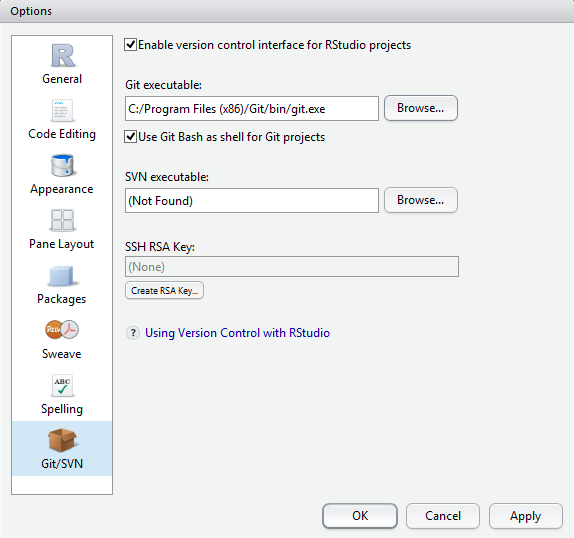
\includegraphics[width=0.6\textwidth,height=\textheight]{../external/images/setup_1_rstudio_git.PNG}

\end{frame}

\begin{frame}{Git basics}
\protect\hypertarget{git-basics}{}

\begin{itemize}[<+->]
\tightlist
\item
  Pull or Fetch: get atest from a repository
\item
  Commit: make a history of your local chanes
\item
  Push: send your commits to a repository
\end{itemize}

\end{frame}

\hypertarget{r}{%
\subsection{R}\label{r}}

\begin{frame}{What is R?}
\protect\hypertarget{what-is-r}{}

\begin{itemize}[<+->]
\tightlist
\item
  R is general purpose programming

  \begin{itemize}[<+->]
  \tightlist
  \item
    Design around \& for statistics
  \item
    ``for and by statisticians''
  \end{itemize}
\item
  R is a collection of tools

  \begin{itemize}[<+->]
  \tightlist
  \item
    Pre-packaged software at your disposal
  \end{itemize}
\item
  R is free (as in beer and speech)

  \begin{itemize}[<+->]
  \tightlist
  \item
    No cost, no restrictions
  \item
    E.g., Microsoft (nee Revolution) R
  \end{itemize}
\item
  R is a functional language

  \begin{itemize}[<+->]
  \tightlist
  \item
    Mathematical functions
  \item
    Pass expressions and functions to and from functions
  \item
    and Turing Complete
  \end{itemize}
\end{itemize}

\end{frame}

\begin{frame}[fragile]{Assignment}
\protect\hypertarget{assignment}{}

\begin{Shaded}
\begin{Highlighting}[]
\CommentTok{# allowed but not preferred}
\NormalTok{a_variable =}\StringTok{ }\DecValTok{10} \OperatorTok{+}\StringTok{ }\DecValTok{1}
\CommentTok{# preferred}
\NormalTok{a_variable <-}\StringTok{ }\DecValTok{10} \OperatorTok{+}\StringTok{ }\DecValTok{1}
\CommentTok{# a bonus}
\DecValTok{10} \OperatorTok{+}\StringTok{ }\DecValTok{1}\NormalTok{ ->}\StringTok{ }\NormalTok{a_variable}
\end{Highlighting}
\end{Shaded}

\end{frame}

\begin{frame}[fragile]{Dots}
\protect\hypertarget{dots}{}

\begin{Shaded}
\begin{Highlighting}[]
\CommentTok{# allowed but not preferred}
\NormalTok{a.variable =}\StringTok{ }\DecValTok{10} \OperatorTok{+}\StringTok{ }\DecValTok{1}
  \CommentTok{## dots have 2 meanings in R, }
    \CommentTok{## with a 3rd in the tidyverse}

\CommentTok{# preferred}
\NormalTok{a_variable <-}\StringTok{ }\DecValTok{10} \OperatorTok{+}\StringTok{ }\DecValTok{1}
\end{Highlighting}
\end{Shaded}

\end{frame}

\begin{frame}[fragile]{``Reserved'' characters}
\protect\hypertarget{reserved-characters}{}

\begin{itemize}[<+->]
\tightlist
\item
  \texttt{c}, \texttt{q}, \texttt{t}, \texttt{C}, \texttt{D},
  \texttt{I}, \texttt{F}, and \texttt{T} (via
  \url{https://www.johndcook.com/blog/r_language_for_programmers/})
\item
  Except that these can be redefined
\end{itemize}

\end{frame}

\begin{frame}{R: Data Structures}
\protect\hypertarget{r-data-structures}{}

\end{frame}

\begin{frame}{R: Data Structures}
\protect\hypertarget{r-data-structures-1}{}

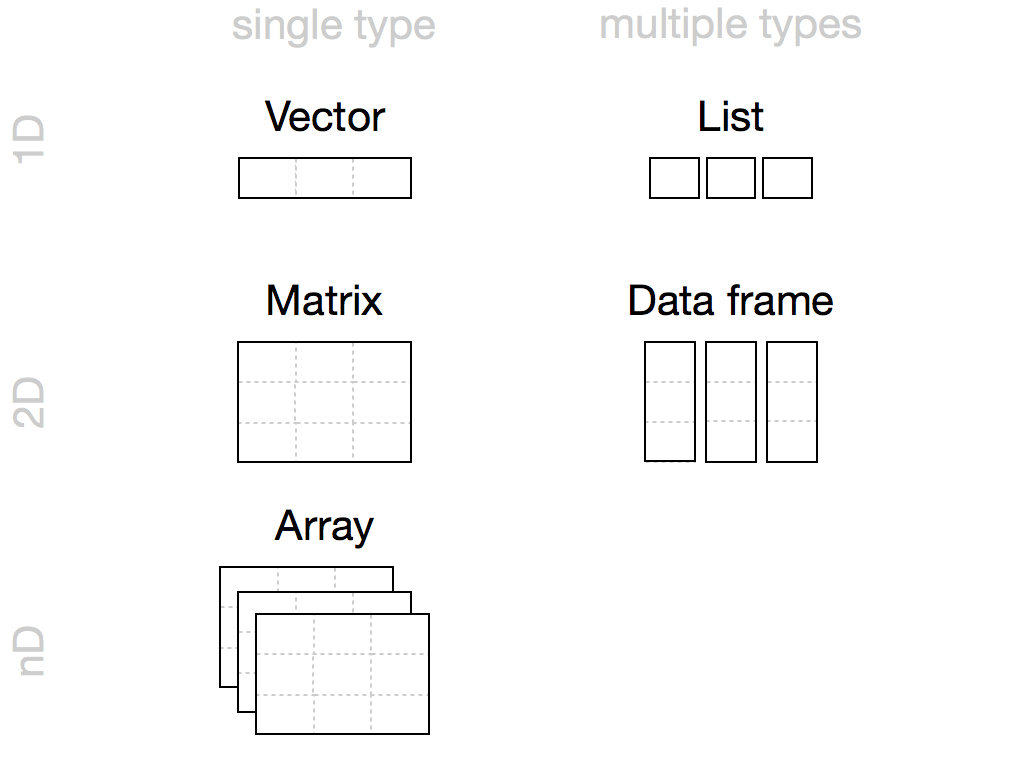
\includegraphics{../external/images/rstudio_datastructs.png} See
\url{https://rstudio-education.github.io/hopr/r-objects.html}

\end{frame}

\begin{frame}

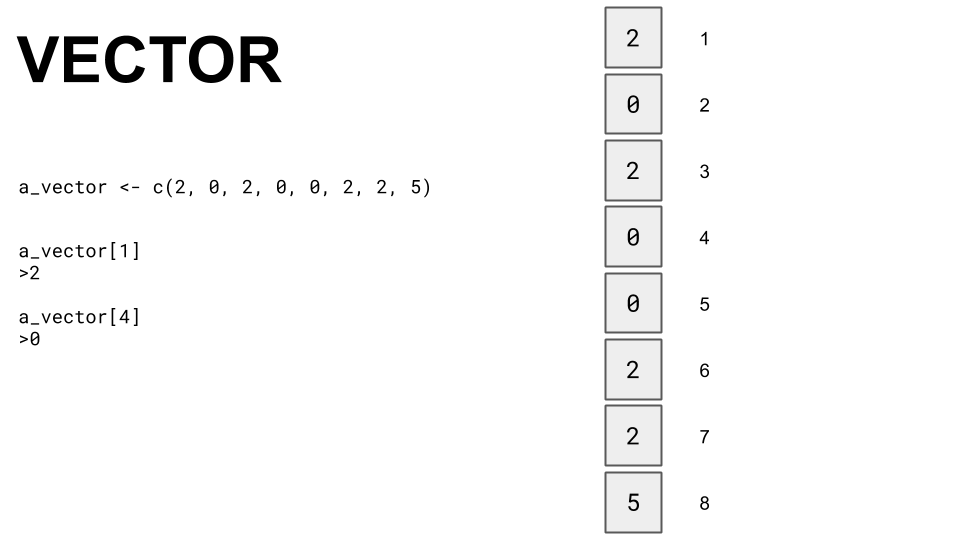
\includegraphics{../external/images/VECTOR.png}

\end{frame}

\begin{frame}

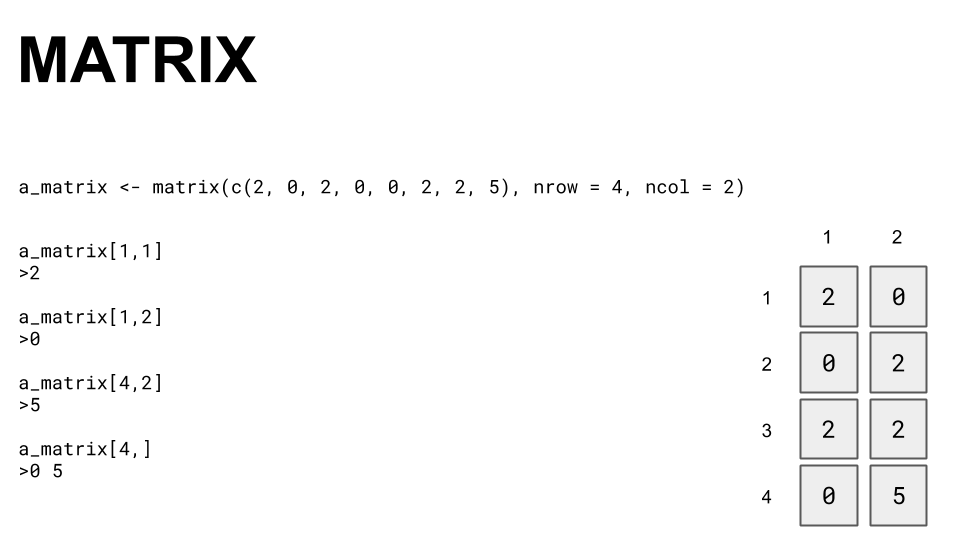
\includegraphics{../external/images/MATRIX.png}

\end{frame}

\begin{frame}

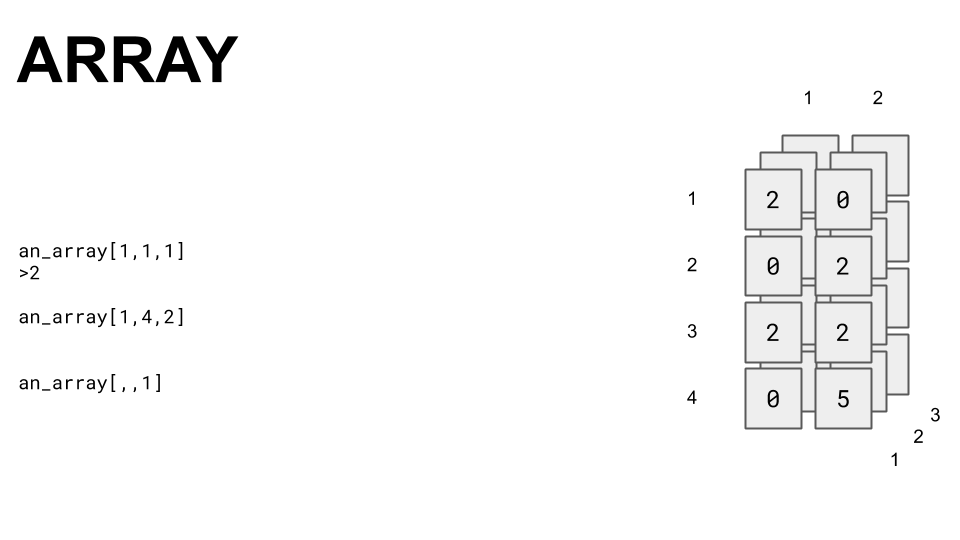
\includegraphics{../external/images/ARRAY_3.png}

\end{frame}

\begin{frame}

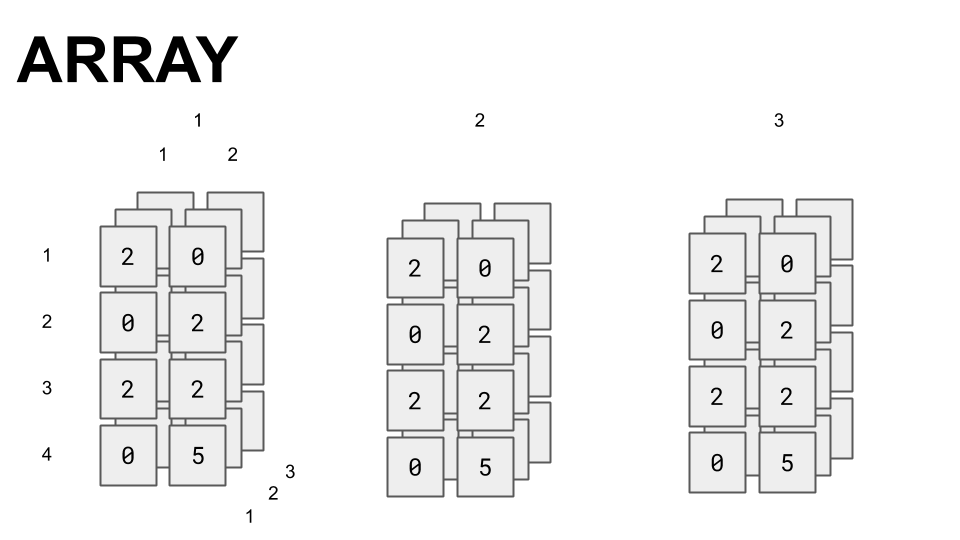
\includegraphics{../external/images/ARRAY_4.png}

\end{frame}

\begin{frame}

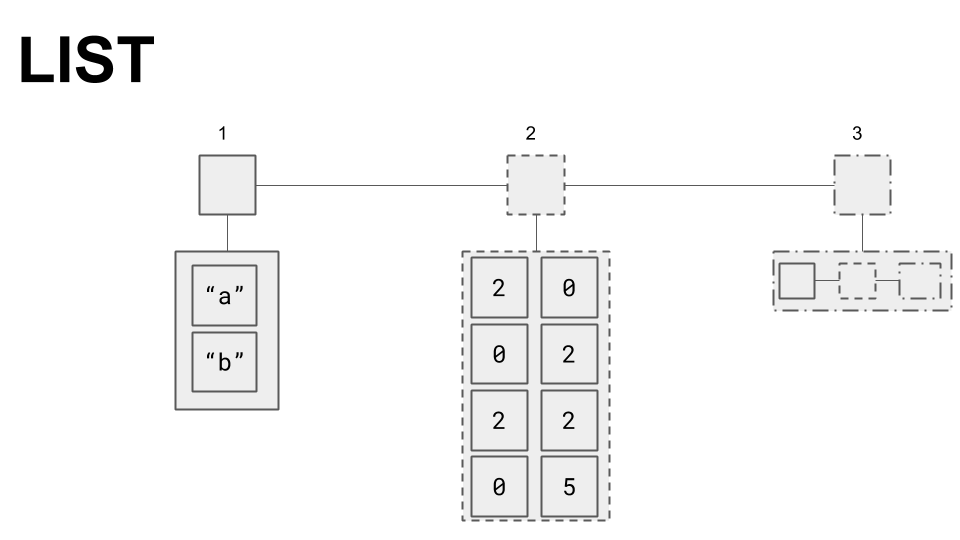
\includegraphics{../external/images/LIST.png}

\end{frame}

\begin{frame}

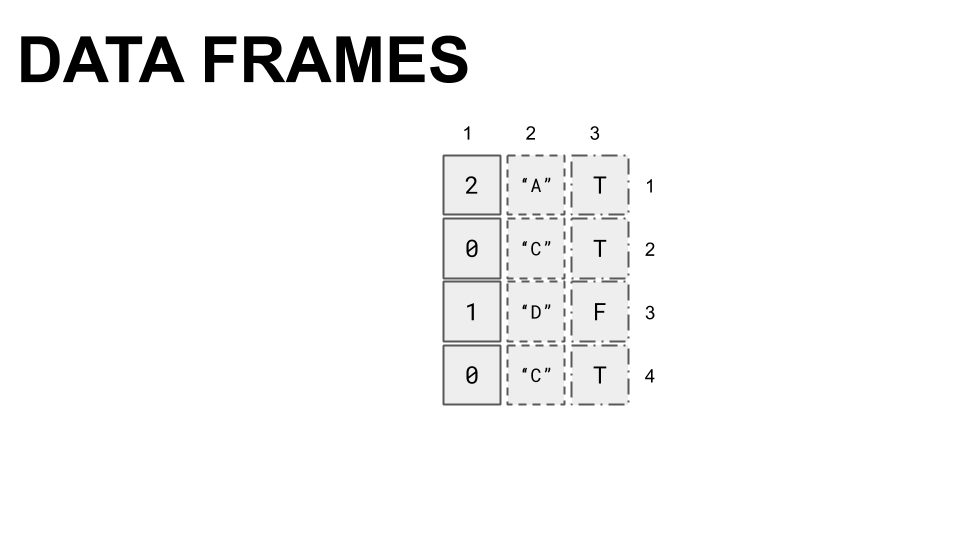
\includegraphics{../external/images/DF.png}

\end{frame}

\begin{frame}[fragile]{R: Data Structures}
\protect\hypertarget{r-data-structures-2}{}

\begin{itemize}[<+->]
\tightlist
\item
  list{[}{[}1{]}{]} or list\$\texttt{name}
\item
  data.frame{[}{[}1{]}{]}{[}1{]} or data.frame{[}1,1{]} or
  data.frame\$\texttt{name}
\end{itemize}

\end{frame}

\begin{frame}[fragile]{R: Data types}
\protect\hypertarget{r-data-types}{}

\begin{itemize}[<+->]
\tightlist
\item
  All of them are here:
  \url{https://cran.r-project.org/doc/manuals/r-release/R-lang.html\#Objects}
\item
  The most common you'll use:

  \begin{itemize}[<+->]
  \tightlist
  \item
    numeric

    \begin{itemize}[<+->]
    \tightlist
    \item
      real or decimal
    \item
      Includes \texttt{NaN}, \texttt{Inf}, \texttt{-Inf}
    \end{itemize}
  \item
    character
  \item
    logical

    \begin{itemize}[<+->]
    \tightlist
    \item
      includes \texttt{NA}, \texttt{T}, \texttt{TRUE}, \texttt{F},
      \texttt{FALSE}
    \end{itemize}
  \end{itemize}
\item
  factor

  \begin{itemize}[<+->]
  \tightlist
  \item
    factors are usually not your friends
  \item
    with \texttt{read.csv()}: \texttt{stringsAsFactors\ =\ F} or convert
    these

    \begin{itemize}[<+->]
    \tightlist
    \item
      \texttt{stringsAsFactors\ =\ F} as default in R 4.0.0
    \end{itemize}
  \item
    or use \texttt{tibble}s in the tidyverse
  \end{itemize}
\end{itemize}

\end{frame}

\begin{frame}[fragile]{R: factor disasters}
\protect\hypertarget{r-factor-disasters}{}

\begin{Shaded}
\begin{Highlighting}[]
\NormalTok{a_numeric_vector <-}\StringTok{ }\KeywordTok{c}\NormalTok{(}\DecValTok{3}\NormalTok{, }\DecValTok{0}\NormalTok{, }\DecValTok{1}\NormalTok{, }\DecValTok{-2}\NormalTok{, }\DecValTok{2}\NormalTok{, }\DecValTok{5}\NormalTok{, }\DecValTok{5}\NormalTok{, }\DecValTok{2}\NormalTok{, }\DecValTok{1}\NormalTok{)}
\NormalTok{(a_numeric_vector }\OperatorTok{+}\StringTok{ }\DecValTok{1}\NormalTok{)}
\end{Highlighting}
\end{Shaded}

\begin{verbatim}
## [1]  4  1  2 -1  3  6  6  3  2
\end{verbatim}

\end{frame}

\begin{frame}[fragile]

\begin{Shaded}
\begin{Highlighting}[]
\NormalTok{a_numeric_vector <-}\StringTok{ }\KeywordTok{c}\NormalTok{(}\DecValTok{3}\NormalTok{, }\DecValTok{0}\NormalTok{, }\DecValTok{1}\NormalTok{, }\DecValTok{-2}\NormalTok{, }\DecValTok{2}\NormalTok{, }\DecValTok{5}\NormalTok{, }\DecValTok{5}\NormalTok{, }\DecValTok{2}\NormalTok{, }\DecValTok{1}\NormalTok{)}
\NormalTok{(a_numeric2factor_vector <-}\StringTok{ }\KeywordTok{as.factor}\NormalTok{(a_numeric_vector))}
\end{Highlighting}
\end{Shaded}

\begin{verbatim}
## [1] 3  0  1  -2 2  5  5  2  1 
## Levels: -2 0 1 2 3 5
\end{verbatim}

\end{frame}

\begin{frame}[fragile]

\begin{Shaded}
\begin{Highlighting}[]
\NormalTok{a_numeric_vector <-}\StringTok{ }\KeywordTok{c}\NormalTok{(}\DecValTok{3}\NormalTok{, }\DecValTok{0}\NormalTok{, }\DecValTok{1}\NormalTok{, }\DecValTok{-2}\NormalTok{, }\DecValTok{2}\NormalTok{, }\DecValTok{5}\NormalTok{, }\DecValTok{5}\NormalTok{, }\DecValTok{2}\NormalTok{, }\DecValTok{1}\NormalTok{)}
\NormalTok{(a_numeric2factor_vector <-}\StringTok{ }\KeywordTok{as.factor}\NormalTok{(a_numeric_vector))}
\end{Highlighting}
\end{Shaded}

\begin{verbatim}
## [1] 3  0  1  -2 2  5  5  2  1 
## Levels: -2 0 1 2 3 5
\end{verbatim}

\begin{Shaded}
\begin{Highlighting}[]
\NormalTok{(}\KeywordTok{as.numeric}\NormalTok{(a_numeric2factor_vector))}
\end{Highlighting}
\end{Shaded}

\begin{verbatim}
## [1] 5 2 3 1 4 6 6 4 3
\end{verbatim}

\begin{Shaded}
\begin{Highlighting}[]
\NormalTok{(}\KeywordTok{as.numeric}\NormalTok{(a_numeric2factor_vector) }\OperatorTok{+}\StringTok{ }\DecValTok{1}\NormalTok{)}
\end{Highlighting}
\end{Shaded}

\begin{verbatim}
## [1] 6 3 4 2 5 7 7 5 4
\end{verbatim}

\end{frame}

\begin{frame}[fragile]

\begin{Shaded}
\begin{Highlighting}[]
\NormalTok{a_numeric_vector <-}\StringTok{ }\KeywordTok{c}\NormalTok{(}\DecValTok{3}\NormalTok{, }\DecValTok{0}\NormalTok{, }\DecValTok{1}\NormalTok{, }\DecValTok{-2}\NormalTok{, }\DecValTok{2}\NormalTok{, }\DecValTok{5}\NormalTok{, }\DecValTok{5}\NormalTok{, }\DecValTok{2}\NormalTok{, }\DecValTok{1}\NormalTok{)}
\NormalTok{(a_numeric2factor_vector <-}\StringTok{ }\KeywordTok{as.factor}\NormalTok{(a_numeric_vector))}
\end{Highlighting}
\end{Shaded}

\begin{verbatim}
## [1] 3  0  1  -2 2  5  5  2  1 
## Levels: -2 0 1 2 3 5
\end{verbatim}

\begin{Shaded}
\begin{Highlighting}[]
\NormalTok{(}\KeywordTok{as.character}\NormalTok{(a_numeric2factor_vector))}
\end{Highlighting}
\end{Shaded}

\begin{verbatim}
## [1] "3"  "0"  "1"  "-2" "2"  "5"  "5"  "2"  "1"
\end{verbatim}

\begin{Shaded}
\begin{Highlighting}[]
\NormalTok{(}\KeywordTok{as.numeric}\NormalTok{(}\KeywordTok{as.character}\NormalTok{(a_numeric2factor_vector)))}
\end{Highlighting}
\end{Shaded}

\begin{verbatim}
## [1]  3  0  1 -2  2  5  5  2  1
\end{verbatim}

\end{frame}

\begin{frame}{Cheatsheet for base R}
\protect\hypertarget{cheatsheet-for-base-r}{}

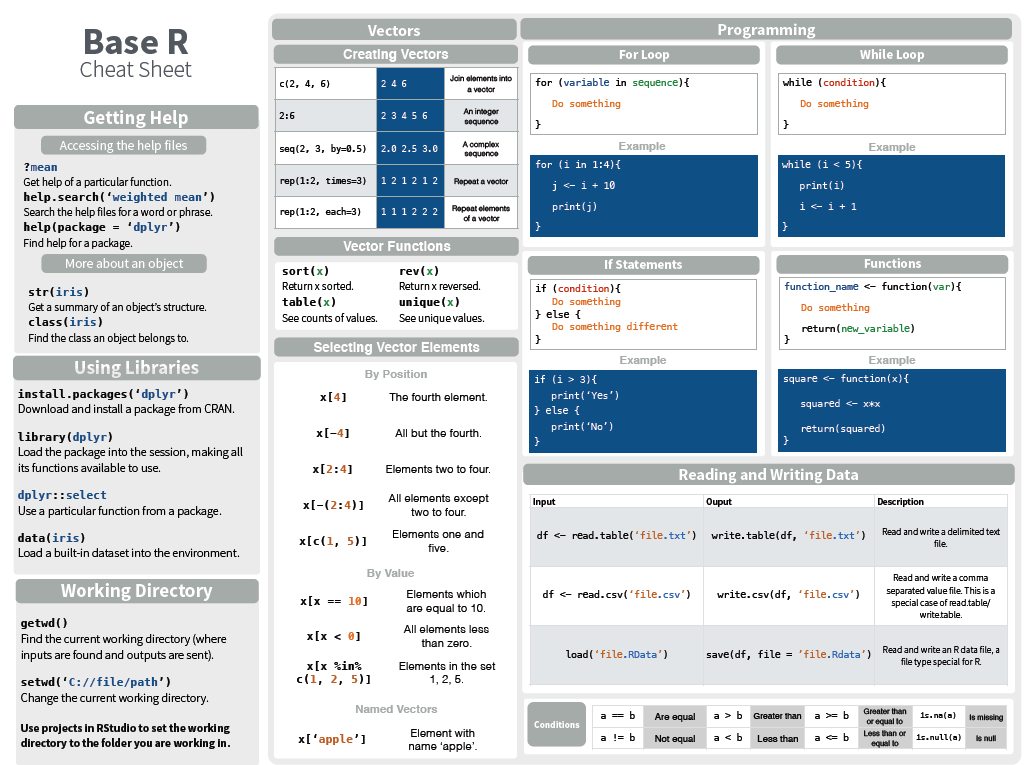
\includegraphics{../external/images/r_cheatsheet_base.PNG} ``Base R''

\end{frame}

\begin{frame}[fragile]{Tidyverse}
\protect\hypertarget{tidyverse}{}

\begin{itemize}[<+->]
\tightlist
\item
  \texttt{tidyverse}: ``an opinionated collection of R packages designed
  for data science {[}that{]} share an underlying design philosophy,
  \textbf{grammar, and data structures.}''

  \begin{itemize}[<+->]
  \tightlist
  \item
    A sublanguage or dialect
  \end{itemize}
\item
  Strongly built around a style:

  \begin{itemize}[<+->]
  \tightlist
  \item
    objects are nouns
  \item
    functions are verbs
  \end{itemize}
\item
  Core packages:

  \begin{itemize}[<+->]
  \tightlist
  \item
    \texttt{ggplot2}, \texttt{dplyr}, \texttt{tidyr}, \texttt{readr},
    \texttt{tibble}, \texttt{stringr}, \texttt{purrr}
  \item
    \url{https://www.tidyverse.org/}
  \end{itemize}
\end{itemize}

\end{frame}

\begin{frame}{tidyverse cheatsheet}
\protect\hypertarget{tidyverse-cheatsheet}{}

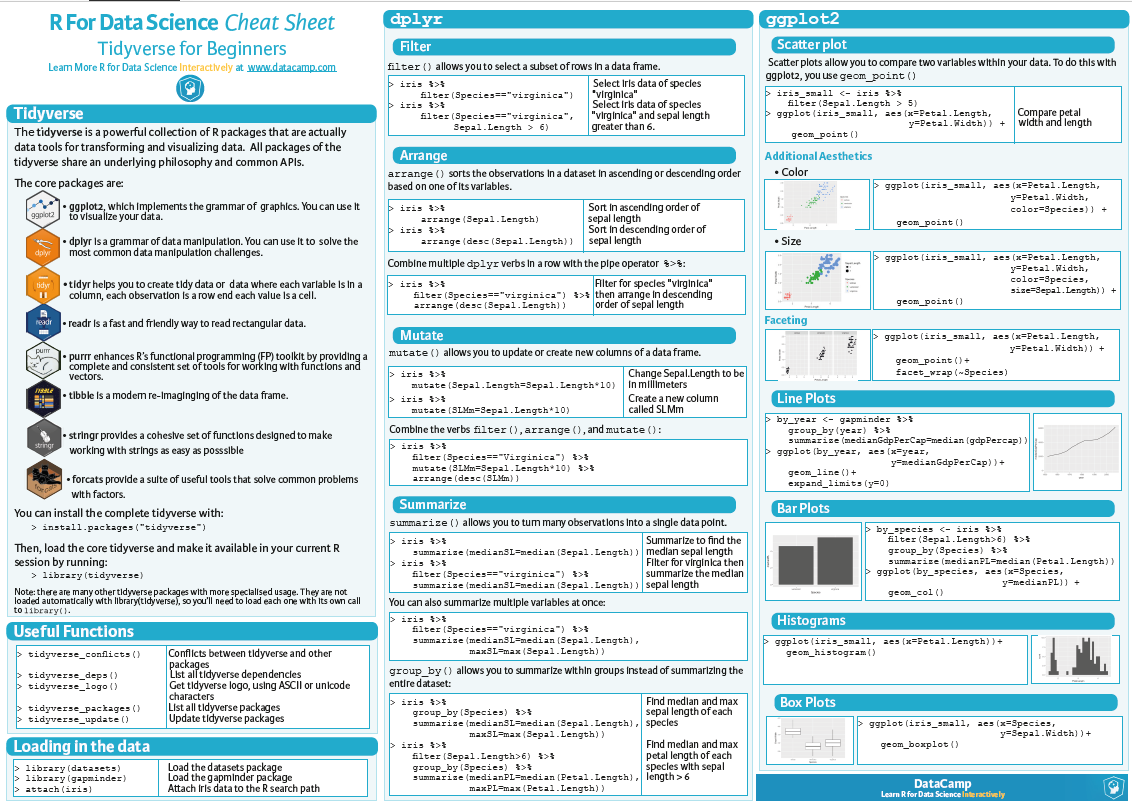
\includegraphics{../external/images/r_cheatsheet_tidy.PNG}

\end{frame}

\hypertarget{rmarkdown}{%
\subsection{RMarkdown}\label{rmarkdown}}

\begin{frame}{RMarkdown}
\protect\hypertarget{rmarkdown-1}{}

\begin{itemize}[<+->]
\tightlist
\item
  A simple markdown language
\item
  Create documents (or slides, websites, books, notebooks, etc\ldots)

  \begin{itemize}[<+->]
  \tightlist
  \item
    \url{https://bookdown.org/yihui/rmarkdown/}
  \item
    See also:
    \url{https://ryanpeek.github.io/2020-02-20-10-tips-to-souping-up-rmarkdown/}
  \end{itemize}
\item
  ``Literate programming''

  \begin{itemize}[<+->]
  \tightlist
  \item
    Text, headers, sections
  \item
    Figures, tables

    \begin{itemize}[<+->]
    \tightlist
    \item
      Code to generate those
    \end{itemize}
  \end{itemize}
\end{itemize}

\end{frame}

\begin{frame}[fragile]{RMarkdown}
\protect\hypertarget{rmarkdown-2}{}

Generate reports:

\begin{itemize}[<+->]
\tightlist
\item
  HTML
\item
  Word
\item
  PDF

  \begin{itemize}[<+->]
  \tightlist
  \item
    With \texttt{LateX}
  \end{itemize}
\end{itemize}

\end{frame}

\begin{frame}{RMarkdown}
\protect\hypertarget{rmarkdown-3}{}

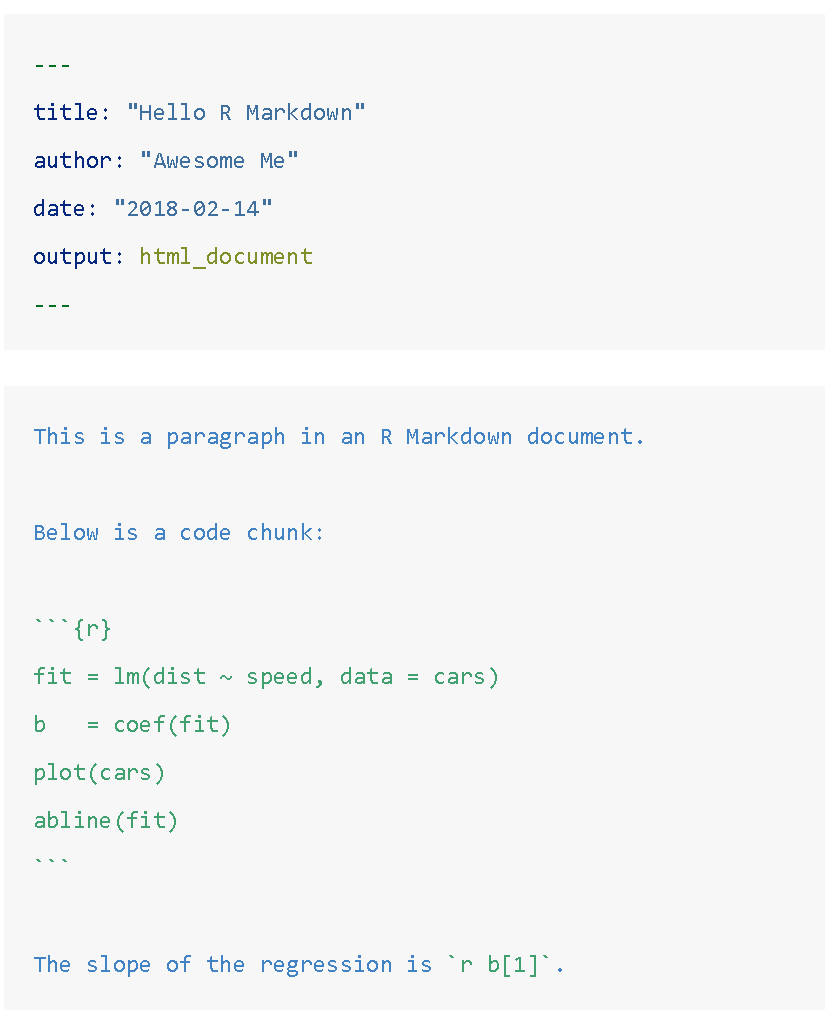
\includegraphics{../external/images/min_markdown.PNG}

\end{frame}

\begin{frame}[fragile]{RMarkdown Don'ts}
\protect\hypertarget{rmarkdown-donts}{}

\begin{itemize}[<+->]
\tightlist
\item
  Don't hardcode values or absolute file paths

  \begin{itemize}[<+->]
  \tightlist
  \item
    see \texttt{here::here()}
  \item
    Use projects (\texttt{.Rproj})
  \end{itemize}
\item
  Don't do complicated or expensive stuff

  \begin{itemize}[<+->]
  \tightlist
  \item
    Database queries
  \item
    Resampling
  \end{itemize}
\end{itemize}

\end{frame}

\hypertarget{all-together}{%
\subsection{All together}\label{all-together}}

\begin{frame}{Within RStudio}
\protect\hypertarget{within-rstudio}{}

\begin{itemize}[<+->]
\tightlist
\item
  Integration with version control (git or SVN)
\item
  R Markdown

  \begin{itemize}[<+->]
  \tightlist
  \item
    Save and execute code
  \item
    Generate high quality reports that can be shared
  \item
    Create presentations (like this one!)

    \begin{itemize}[<+->]
    \tightlist
    \item
      See
      \url{https://github.com/derekbeaton/Workshops/tree/master/Misc/R_RStudio_Workflow}
    \end{itemize}
  \end{itemize}
\item
  Python, D3 (JavaScript), SQL, Shiny, LaTeX, HTML/CSS
\item
  And so much more
\end{itemize}

\end{frame}

\hypertarget{part-2-working-with-data}{%
\section{Part 2: Working with data}\label{part-2-working-with-data}}

\begin{frame}{Part 2: Working with data}

We'll move to R scripts and another RMarkdown document

\end{frame}

\begin{frame}{Before we do}
\protect\hypertarget{before-we-do}{}

\begin{itemize}[<+->]
\tightlist
\item
  Today's data come from
  \url{https://sharlagelfand.github.io/opendatatoronto/index.html}
\item
  Today's workshop is a subset of
  \url{https://github.com/jennyrieck/workshops/tree/master/2019_Rstudio_Magic}
\item
  See ``say hello to your Data'':
  \url{https://djnavarro.github.io/robust-tools/hello/\#1}
\item
  Feedback form for today: \url{https://forms.gle/R9AB1Wkzhb23KHGU9}
\end{itemize}

\end{frame}

\end{document}
